\documentclass[aps,twocolumn,10pt,nofootinbib]{revtex4-2}

\usepackage{dcolumn}% Align table columns on decimal point
\usepackage[T1]{fontenc}
\usepackage{amsmath}
\usepackage[detect-all]{siunitx}
\usepackage{etoolbox}

\usepackage{placeins}

\usepackage{graphicx}
\usepackage{amssymb}
\usepackage{enumitem}
\usepackage{physics}
% nolist: acronyms are still defined (and expanded on first use), but the
% list is not typeset. It also implies nohyperlinks, so \ac{} produces
% plain text rather than links into the list.
\usepackage[nolist]{acronym}
\usepackage[pdftex,dvipsnames]{xcolor}
\usepackage{xargs}
\usepackage{mathtools}
\usepackage{bm}
\usepackage{verbatim}
\usepackage[hidelinks]{hyperref}
\usepackage{nameref}

\usepackage{comment}


\usepackage{todonotes}
% Visible editorial notes: unresolved hardware details or proposed analyses.
\newcommand{\reviewnote}[1]{\par\smallskip{\color{Purple}\noindent\textbf{Draft note:} #1\par}\smallskip}



\begin{document}
%\listoftodos

\title{miniLISA: Design and Component Noise Model of an Optical Time-Delay Interferometry Testbed}% Force line breaks with \\
% \thanks{A footnote to the article title}%

\author{Author list to be confirmed}
    % \email{reid.ferguson@aei.mpg.de}
 % \altaffiliation[Also at ]{Physics Department, XYZ University.}%Lines break automatically or can be forced with \\
% \author{Second Author}%
%  \email{Second.Author@institution.edu}
\affiliation{%
Max Planck Institute for Gravitational Physics
}%
\date{\today}% It is always \today, today,
             %  but any date may be explicitly specified

\begin{abstract}
We describe miniLISA, a laboratory testbed combining optical laser signals, FPGA-based electronic propagation delays, and independently referenced spacecraft phasemeters. The design reproduces the laser-noise structure of LISA's one-way measurements, a reduced sideband clock-transfer model, and electronically injected gravitational-wave phase responses. We relate the hardware signals to the interferometric measurement model and propagate measured electronic and sideband-difference spectra together with a prospective detector-noise calculation through a static, clock-corrected Michelson observable. The resulting component budget is conditional on ideal laser- and clock-noise cancellation and on the assumed origin of the sideband-difference noise. We identify delay knowledge, differential board timing, and clock-transfer characterization as remaining requirements for testing the assembled optical system, and outline the extension to time-dependent delays.
\end{abstract}

%\keywords{Suggested keywords}%Use showkeys class option if keyword
                              %display desired
\maketitle

%\tableofcontents

\section{Introduction}
Gravitational waves provide a unique observational window into astrophysical and cosmological phenomena. Since the first direct detection in 2015 \cite{abbott2016observation}, the \ac{LVK} collaboration has observed dozens of compact binary coalescences in the 10 Hz to 10 kHz frequency band \cite{}. Accessing gravitational waves at millihertz frequencies requires a space-based detector to overcome terrestrial seismic and Newtonian noise and to provide sufficiently long interferometric baselines. The \ac{LISA}, a joint ESA–NASA mission scheduled for launch in the mid-2030s, is designed to operate in the 0.1 mHz to 1 Hz band \cite{colpi_lisa_2024}.

The \ac{LISA} constellation consists of three spacecraft arranged in an approximately equilateral triangle with arm lengths of about 2.5 million km. Laser beams exchanged between the spacecraft form a constellation-scale interferometer. Unlike ground-based detectors with effectively equal arms, the LISA arm lengths vary by up to about 1.2\% due to orbital motion, preventing direct cancellation of laser frequency noise. Although cavity pre-stabilisation reduces laser frequency noise substantially, it remains several orders of magnitude above the displacement noise budget required for gravitational-wave detection \cite{}. To suppress this noise, \ac{TDI} has been developed as a post-processing technique that synthesizes virtual equal-arm interferometers by appropriately time-shifting and combining phasemeter measurements.

In addition to laser frequency noise, LISA measurements are affected by clock noise originating from the independent \acp{USO} carried by each spacecraft. Since all phase measurements are referenced to these clocks, timing jitter couples directly into the measured heterodyne beatnotes. Space-qualified \acp{USO} achieve Allan deviations of order $10^{-13}$ at one-second averaging times \cite{weaver2010performance}, which is insufficient for the picometer-level test-mass position sensitivity required by LISA. To mitigate this effect, LISA employs additional clock-noise transfer measurements—implemented via modulation sidebands exchanged between spacecraft.
 
%Experimental tests of \ac{TDI}, including representative inter-spacecraft delays implemented in hardware, have been performed in several laboratory setups. These experiments have demonstrated laser-frequency noise suppression, clock-noise suppression, and electronic delay implementations on the order of seconds. The present work builds upon these efforts by extending such testbeds toward a more integrated hardware-in-the-loop configuration and by enabling the injection of physically consistent gravitational-wave strain signals into the measurement chain.

\ac{TDI} has been extensively studied theoretically [] and validated through numerical simulations []. Such simulations, however, generate the measurements from the same model that the analysis pipeline assumes, and therefore test the implementation of the model rather than the model itself. Testing the model requires data produced independently of it, by a physical realization of the measurement chain. Experimental verification of this kind is still developing.

A major milestone was the \ac{UFLIS}, which demonstrated that second-generation \ac{TDI} combinations can suppress laser frequency noise by ten orders of magnitude [4]. The work presented here is a continuation of the \ac{UFLIS} approach with the addition of independent clock sources for each spacecraft, largely enabled by developments in FPGA technology. Other experiments have also contributed important demonstrations relevant to \ac{TDI} and clock-noise removal. The setup by de Vine et al. demonstrated laser frequency noise suppression at a level of roughly nine orders of magnitude and clock-phase noise suppression of about four orders, although without accounting for realistic photon light-travel times. The LISA on Table experiment in Paris more recently demonstrated laser-noise removal using direct digital synthesis (DDS)-generated signals and electronically imposed delays. The Hexagon experiment in Hannover has provided strong results for clock-noise removal and synchronization.

Here, we present an overview of an ongoing effort to develop a \ac{TDI} testbed that combines realistic laser frequency noise, programmable delay lines, and independent clock sources within a single experimental framework. The testbed focuses on reproducing the dominant noise couplings of the LISA metrology system—specifically, laser frequency noise and clock noise—while preserving the structure imposed by unequal and time-dependent delays. Crucially, the same delay lines that impose the inter-spacecraft light-travel times also allow physically consistent gravitational-wave strain signals to be injected directly into the measurement chain. The testbed can therefore be used not only to demonstrate noise suppression, but to verify that a known gravitational-wave signal survives \ac{TDI} processing of hardware-generated data with the expected amplitude and phase.

An initial purely electrical implementation centered around \ac{FPGA}-based digital delay lines has already been demonstrated in Ferguson et al. [REF]. The developments discussed here extend that architecture by incorporating an optical front-end with physically representative laser noise and independently running spacecraft clocks. This preserves the essential timing, noise, and signal-propagation structure of the LISA one-way measurements, allowing \ac{TDI} combinations and clock-noise calibration to be formed entirely from hardware-generated data. The goal of this work is to realize a laboratory-scale analog of the LISA inter-satellite metrology system—a “miniLISA”—that bridges the gap between idealized software simulations and the flight instrument, and provides a controlled environment for testing the robustness of \ac{TDI} to instrumental non-idealities and realistic gravitational-wave signal injection.

The goal is for both noise sources, once processed through \ac{TDI} and clock-noise calibration, to be reduced below the level required for gravitational-wave signal recovery across the core LISA measurement band.

The article is divided as follows:% in section \ref{}, we give an overview of the \ac{LISA} measurement system, and in section \ref{}, we describe our experimental setup to replicate said measurement system in the lab with a focus on aspects relevant to \ac{TDI} and clock noise removal. In section \ref{Comparison}, analyze the expected performance of the setup. In section \ref{}, we discuss the limitations and future prospects in replicating the \ac{LISA} measurement system in this manner, and in section \ref{}, we conclude.

\section{LISA Interferometric Detection System}
\label{sec:modelling}
We now describe the LISA \ac{IDS} and present a mathematical model of the noises. We specifically focus on relevant elements for laser frequency noise and \ac{USO} jitter propagation and coupling. %Although in the real case, the clock noise suppression procedure relies on the use of the reference interferometer, here we focus on the interspacecraft interferometer as the test mass and reference interferometers are currently not included in our setup. 


\subsection{Interferometric Phase Measurements}
Each of the three identical LISA satellites carries two lasers on board. We refer to one as the local laser and the other as the adjacent laser. These two laser fields interfere on the test-mass and reference interferometers on the two optical benches of the spacecraft. In addition, the local laser interferes with the laser received from a distant spacecraft on the science interferometer. It is this science interferometer that encodes the gravitational-wave signal by measuring fluctuations in the spacecraft-to-spacecraft distance, while the test mass interferometer will measure the spacecraft-to-test mass displacement. In Figure \ref{fig:armlink} (a), a simplified LISA two-way armlink involving only the science interferometer is shown.

We begin by writing the optical phase of the laser field originating from \ac{MOSA} $ij$ on spacecraft $i$ as a function of a common modelling time $t$:
\begin{equation}\label{total_phase}
    \Phi_{ij}(t) = \nu_{ij} t + \delta \phi_{ij}(t),
\end{equation}
where $\nu_{ij}$ denotes the nominal carrier frequency and $\delta \phi_{ij}(t)$ represents the intrinsic laser phase noise. Throughout this section, phases are expressed in cycles, frequencies in Hz, and clock errors in seconds. Capital $\Phi$ denotes total phase, while $\delta\phi$ denotes phase fluctuations about the nominal linear evolution. Nominal carrier and modulation frequencies are assumed constant. Laser phase fluctuations carry two MOSA indices here, $\delta\phi_{ij}$. The one-laser-per-spacecraft testbed uses the corresponding single-index notation $\delta\phi_i$. We define the local clock reading by $t_i=t+q_i(t)$; thus $q_i$ is a timing error, while $\dot q_i$ is a fractional-frequency error. The explicit noise-coupling equations below retain terms linear in these errors and use nominal, constant beatnote coefficients. Differences between spacecraft proper times are not modelled here.


\begin{figure*}
    \centering
    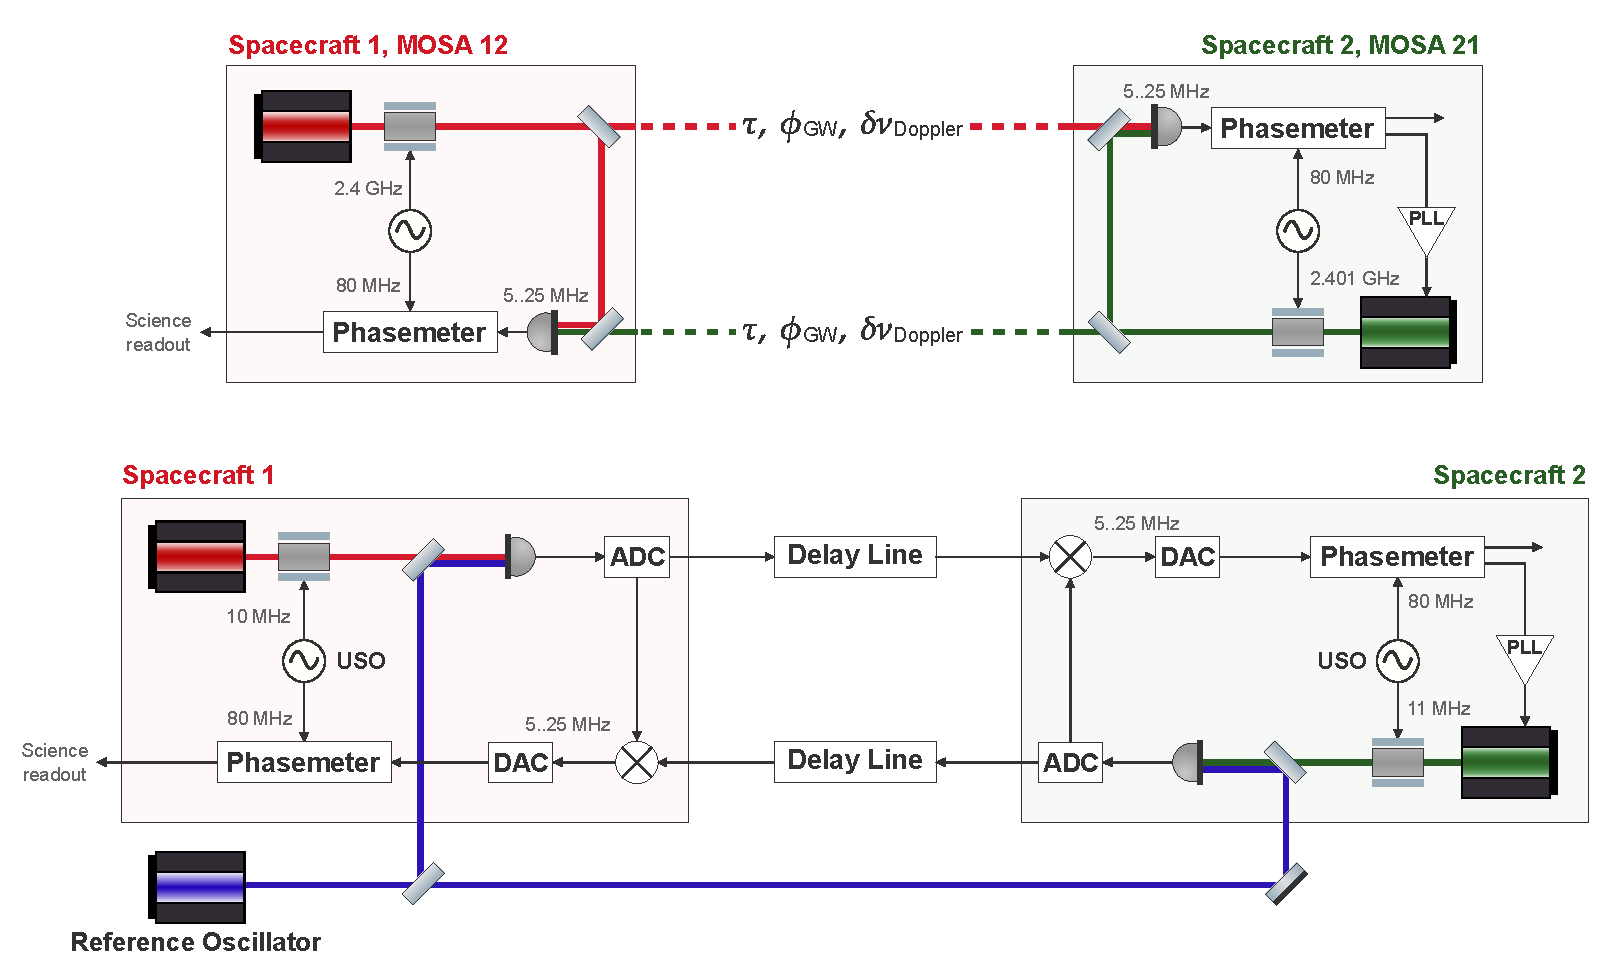
\includegraphics[width=\linewidth]{images/LISAarm-analysis.pdf}
    \caption{A comparison of the two-way links as implemented in LISA (upper) and the testbed (lower). The upper panel shows the conceptual LISA configuration: the laser on Spacecraft 1 (MOSA 12) is phase-modulated at approximately 2.4 GHz using the local USO and transmitted to Spacecraft 2 (MOSA 21). The received beam interferes with the local laser, producing heterodyne beat notes in the MHz range that contain gravitational-wave phase fluctuations, Doppler shifts due to orbital motion, and laser frequency noise. These beat notes are tracked by the phasemeter, which is clocked by the onboard 80 MHz sampling reference derived from the USO. The lower panel depicts the laboratory implementation of the same signal topology. Instead of physical light propagation over millions of kilometres, the inter-spacecraft delay is emulated electronically using digital delay lines between ADC and DAC stages. A common reference oscillator is used to downconvert the laser fields from hundreds of terahertz to tens of megahertz, which can then be sampled by the delay line \acp{ADC}. The actual LISA-like heterodyne beat notes are created in the mixers.}
    \label{fig:armlink}
\end{figure*}


Each of the laser fields is phase-modulated using an \ac{EOM} driven by the local USO. This is used to imprint sidebands on the laser field that carry the USO timing noise $q_i(t)$, with modulation phase noise $\nu^m_{ij}q_i(t)$. Since there is only one \ac{USO} per spacecraft, clock noise carries a single spacecraft index.

The modulation frequency $\nu^m_{ij}$ will be about 2.4 GHz, which is upconverted from the \ac{USO} via a \ac{PLL} synthesizer, preserving its noise with high fidelity. For the adjacent and opposing \ac{MOSA}s $ik$ and $ji$ respectively, the corresponding modulation frequency differs by 1 MHz, so 2.401 GHz, such that the sideband–sideband beat notes are offset by 1 MHz from the carrier–carrier beat note. The modulation depth $m= 0.53$ should be a fair trade-off between optical power in the carrier-carrier versus the sideband-sideband beat notes. The clock noise transfer scheme and its suppression are discussed further in the subsection \ref{clock noise}. Lower frequency offset sidebands will also be used for pseudo-random ranging and data transfer between the satellites, but are not covered here.

%
As the beam propagates from \ac{MOSA} $ij$ toward spacecraft $j$ and its \ac{MOSA} $ji$, it accumulates phase contributions from Doppler shifts due to the relative spacecraft motion and from gravitational waves integrated along the arm. Following the separation of background propagation and GW perturbations in \cite{bayle_unified_2023}, we write
\begin{equation}
    d^{\mathrm{tot}}_{ji}(t)=d_{ji}(t)+H_{ji}(t).
\end{equation}
Here $d_{ji}(t)$ is the background propagation time, which can vary slowly with the constellation breathing, and $H_{ji}(t)$ is its GW-induced perturbation. The first index denotes the receiving spacecraft and the second the emitting spacecraft. In the common-time model used here, this is a propagation-time decomposition; we do not include the transformations between spacecraft proper times contained in the proper pseudorange of \cite{bayle_unified_2023}. We define the delay operator using only the background propagation time,
\begin{equation}
    \mathbf D_{ji}x(t)=x\!\left(t-d_{ji}(t)\right).
\end{equation}
Applying the total propagation time to Eq.~\eqref{total_phase} and expanding to first order gives
\begin{align*}
    \Phi_{ij}\!\left(t-d_{ji}(t)-H_{ji}(t)\right)
    \simeq{}&\nu_{ij}\left[t-d_{ji}(t)\right]\\
    &+\mathbf D_{ji}\delta\phi_{ij}(t)
    -\nu_{ij}H_{ji}(t),
\end{align*}
where the product $H_{ji}\mathbf D_{ji}\delta\dot\phi_{ij}$ of the GW perturbation and laser-frequency noise has been neglected. We therefore introduce the GW phase contribution
\begin{equation}\label{eq:gw_phase}
    \delta\phi^{\mathrm{GW}}_{ji}(t)=-\nu_{ij}H_{ji}(t).
\end{equation}
To this order, the received total phase is $\mathbf D_{ji}\Phi_{ij}(t)+\delta\phi^{\mathrm{GW}}_{ji}(t)$: the GW signal is an additive phase contribution, separate from the background delay operator. For constant $\nu_{ij}$, the corresponding frequency fluctuation is $\delta\dot\phi^{\mathrm{GW}}_{ji}=-\nu_{ij}\dot H_{ji}$.

At spacecraft $j$, the received field $i$ interferes with the local laser field of phase $\Phi_{ji}(t)$ on a photodetector. The resulting heterodyne signal contains both the carrier–carrier beat note and the sideband–sideband beat notes. Additional cross terms lie outside the heterodyne range of the phasemeter, 5 to 25 MHz.

The electrical signal from the photodetector is then digitized by the \ac{PMS} front-end electronics. The sampling process introduces a coupling of the local USO timing error $q_j(t)$ into the measured phase. With $t_j=t+q_j(t)$ and a signed distant-minus-local beat frequency, the first-order sampling contribution is minus the beat frequency times $q_j(t)$. We define the nominal carrier coefficient
\begin{equation}
    \alpha_{ji}=\Delta\nu_{ji}=\nu_{ij}-\nu_{ji}.
\end{equation}
After subtracting the nominal phase evolution, we can write the phase fluctuations of the carrier-carrier beat note measurement
\begin{equation}\label{Main_LISA_eq}
    \begin{aligned}
    \delta\phi^{\text{c}}_{ji}(t)={}&\mathbf D_{ji}\delta\phi_{ij}(t)-\delta\phi_{ji}(t)\\
    &+\delta\phi^{\mathrm{GW}}_{ji}(t)-\alpha_{ji}q_j(t).
    \end{aligned}
\end{equation}

The signal is then passed to \acp{DPLL}, which demodulate the carrier and sideband beat notes and extract the phase fluctuations of each. So the phasemeter produces three measurements from the science interferometer photodetector that are of interest to us: the carrier beat note, which contains the gravitational-wave signal of interest, and the sideband readouts, which are used for clock jitter suppression. For all measurement readouts, we adopt the LISA convention that phases are written as “distant minus local.”\footnote{In practice, the sign depends on the frequencies constituting the beat note as the phasemeter only sees the absolute value of the difference. However, we can always get this knowledge from the frequency planning.} The carrier phase measurement recorded on spacecraft $j$ for the light received from spacecraft $i$ is
\begin{align}
    \text{sci}^{\text{c}}_{ji}(t) = & \mathbf{D}_{ji}\delta \phi_{ij}(t)-\delta \phi_{ji}(t)-\alpha_{ji}q_j(t)\nonumber\\[3pt]
    &+\delta\phi^{\mathrm{GW}}_{ji}(t)+N^{\text{c}}_{ji}(t)\nonumber\\[3pt]
    &-\frac{\nu_0}{c}\left(\mathbf{n}_{ij}\cdot \mathbf{D}_{ji}\bm{\Delta}_{ij}(t)+\mathbf{n}_{ji}\cdot\bm{\Delta}_{ji}(t)\right),
\end{align}
The term $N^{\mathrm{c}}_{ji}(t)$ represents combined readout noise from optical path-length fluctuations and electronics. The vectors $\bm{\Delta}_{ij}(t)$ are optical-bench displacements in metres. The unit vector $\mathbf n_{ji}$ points along the incoming beam from spacecraft $i$ to spacecraft $j$, and $\mathbf n_{ij}=-\mathbf n_{ji}$ in the geometry used for these displacement terms. We use a common nominal optical frequency $\nu_0$ in all displacement couplings, neglecting relative optical-frequency offsets there; the distinct frequencies are retained in the heterodyne clock coefficients. Thus $\nu_0/c$ converts a one-way displacement into phase in cycles.

%\Delta\omega^{\mathrm{sb}}_{ij}t+ 
The corresponding upper sideband–sideband beat note readout can be written as
\begin{align}\label{SB_meas}
    \text{sci}^{\mathrm{sb,+}}_{ji}(t)=&
    \mathbf{D}_{ji}\delta\phi_{ij}(t)- \delta\phi_{ji}(t)- \gamma_{ji}\, q_j(t)\nonumber\\[3pt]
    &+\delta\phi^{\mathrm{GW}}_{ji}(t)+N^{\mathrm{sb,+}}_{ji}(t)\nonumber\\[3pt]
    &-\frac{\nu_0}{c}\left(\mathbf{n}_{ij}\cdot \mathbf{D}_{ji}\bm{\Delta}_{ij}(t)+\mathbf{n}_{ji}\cdot\bm{\Delta}_{ji}(t)\right)
    \nonumber\\[3pt]
    &+\nu^m_{ij} \mathbf{D}_{ji} q_i(t)- \nu^m_{ji} q_j(t).
\end{align}
The sideband clock coupling coefficient is
\begin{equation}
    \gamma_{ji} =\Delta\nu_{ji}+\nu^m_{ij}-\nu^m_{ji}=\Delta\nu_{ji}+\Delta\nu^m_{ji}= \Delta\nu_{ji}^{\mathrm{sb,+}}.
\end{equation}
Again, the term $N^{\mathrm{sb,+}}_{ji}(t)$ represents stochastic readout noise specific to the upper sideband measurement. The lower sideband has the same laser phase noise but the opposite sign for each modulation contribution, including the modulation part of the beatnote coefficient. We show the upper sideband explicitly. Relative corrections of order $\nu^m/\nu_0$ to the displacement coupling are neglected. We also neglect the relative correction $\nu^m_{ij}/\nu_{ij}$ to the GW coupling: the exact upper-sideband contribution at this order is $-(\nu_{ij}+\nu^m_{ij})H_{ji}$, approximated here by the same $\delta\phi^{\mathrm{GW}}_{ji}$ as in the carrier. This makes the retained GW term common to the carrier and both sidebands. 

For completeness, we also write out the reference and test mass interferometer readings on \ac{MOSA} $ji$
\begin{align}
\text{tm}_{ji}(t)= &
\delta\phi_{jk}(t)-\delta\phi_{ji}(t)
+\beta_{ji}q_j(t)+\mu_{j}(t)+N^{\text{tm}}_{ji}(t)\nonumber\\[3pt]
&+\frac{2\nu_0}{c}
\mathbf{n}_{ji}\cdot\left(\bm{\delta}_{ji}(t)-\bm{\Delta}_{ji}(t)\right),\\[5pt]
\text{ref}_{ji}(t)&=\delta\phi_{jk}(t)-\delta\phi_{ji}(t)+\beta_{ji}q_j(t)+\mu_{j}(t)+N^{\text{ref}}_{ji}(t).
\end{align}
Here we have introduced the fiber noise $\mu_{j}$ coming from the optical fiber that exchanges the local and adjacent laser fields between \ac{MOSA} $ji$ and \ac{MOSA} $jk$ . This term is typically referred to as the backlink noise. We have assumed it to be independent of the direction of propagation of the optical beams within. The vector $\bm{\delta}_{ji}$ is the test-mass displacement in metres, including displacement produced by acceleration noise; it is not itself an acceleration. With the same sampling convention, the reference and test-mass clock coefficient is
\begin{equation}
    \beta_{ji}=\nu_{ji}-\nu_{jk}.
\end{equation}
It has the opposite sign to the adjacent-minus-local beat frequency, which explains the plus sign multiplying $\beta_{ji}q_j$ in the readouts.

In reality, the beat notes will contain many more noise sources, for example, the tilt-to-length coupling or \ac{ADC} noise. Since our testbed does not include the test mass or reference interferometers, the associated optical-bench motion, backlink fiber noise, and test mass acceleration noise terms will not be considered in the following sections.


\subsection{Laser Noise and \ac{TDI}}

In the LISA measurement system, laser frequency noise is first reduced onboard by locking one laser to an optical resonator and phase-locking the remaining lasers to this pre-stabilized reference with fixed frequency offsets. The last step ensures that all heterodyne beat notes remain within the phasemeter bandwidth while maintaining coherent phase relationships between spacecraft. However, residual laser frequency noise remains many orders of magnitude above the displacement sensitivity requirement and must be suppressed in post-processing. \ac{TDI} achieves this by forming linear combinations of one-way phase measurements and appropriately delayed copies thereof, effectively synthesizing an equal-arm interferometer in post-processing.

Because the inter-spacecraft separations vary in time due to orbital motion, the light-travel times entering the delay operators are time-dependent. As a result, delay operators do not commute, and first-generation \ac{TDI} combinations do not yield exact cancellation. Second-generation \ac{TDI} combinations account for time-varying delays and achieve exact cancellation for delays that are approximately linear in time.

Accurate knowledge of the delays is essential, as an error $\delta d$ in the applied delay leads to residual laser noise proportional to the time derivative of the laser phase noise. This sets the requirement on delay knowledge to approximately one meter, motivating LISA’s dedicated ranging system.

Before \ac{TDI} is implemented, intermediary variables are constructed. The reference and test-mass interferometer readings remove optical-bench displacement noise, as discussed in \cite{otto2012tdi,tinto2018time}. To make the signs explicit, define
\begin{align*}
    T_{ji}&=\text{tm}_{ji}-\text{ref}_{ji},\\
    \xi_{ji}&=\text{sci}^{\mathrm c}_{ji}
    -\frac12\left(T_{ji}+\mathbf D_{ji}T_{ij}\right).
\end{align*}
Within the common-optical-frequency approximation above, the bench terms cancel, leaving the test-mass contribution
\begin{equation*}
    M_{ji}=-\frac{\nu_0}{c}\left[
    \mathbf n_{ji}\cdot\bm\delta_{ji}(t)
    +\mathbf D_{ji}\!\left(\mathbf n_{ij}\cdot\bm\delta_{ij}(t)\right)
    \right].
\end{equation*}
The following equations omit readout noises. Reciprocal backlink noise cancels in the local reference difference
\begin{equation*}
    z_{ji}=\frac12\left(\text{ref}_{ji}-\text{ref}_{jk}\right)
    =\delta\phi_{jk}-\delta\phi_{ji}+\beta_{ji}q_j.
\end{equation*}
For cyclic triples $(i,j,k)=(1,2,3),(2,3,1),(3,1,2)$, the intermediate variables can then be defined as
\begin{align*}
    \eta_{ji}&=\xi_{ji}-z_{ji}\\
    &=\mathbf D_{ji}\delta\phi_{ij}(t)-\delta\phi_{jk}(t)
    -(\alpha_{ji}+\beta_{ji})q_j(t)\\
    &\quad+\delta\phi^{\mathrm{GW}}_{ji}(t)+M_{ji}(t),\\[3pt]
    \eta_{ij}&=\xi_{ij}+\mathbf D_{ij}z_{ji}\\
    &=\mathbf D_{ij}\delta\phi_{jk}(t)-\delta\phi_{ij}(t)
    -\alpha_{ij}q_i(t)\\
    &\quad+\mathbf D_{ij}\!\left[\beta_{ji}q_j(t)\right]\\
    &\quad+\delta\phi^{\mathrm{GW}}_{ij}(t)+M_{ij}(t).
\end{align*}
Here $M_{ij}$ is obtained by exchanging $i$ and $j$ in $M_{ji}$. These combinations reduce the number of independent laser phase noises from six to three, retaining $\delta\phi_{12}$, $\delta\phi_{23}$ and $\delta\phi_{31}$, while removing the optical-bench displacement terms. The construction introduces an asymmetry between the two link orientations.

Further, as an example, a commonly used first-generation Michelson-type \ac{TDI} observable synthesised at spacecraft $i$ is the $X_i$ combination, which can be written as
\begin{align}
X_i(t) ={}&
\Bigl[(\eta_{ik}(t) + \mathcal{D}_{ik}\eta_{ki}(t))+
\mathcal{D}_{ik}\mathcal{D}_{ki}(\eta_{ij}(t) + \mathcal{D}_{ij}\eta_{ji}(t))
\Bigr]\nonumber\\[3pt]
&-\Bigl[(\eta_{ij}(t) + \mathcal{D}_{ij}\eta_{ji}(t))+
\mathcal{D}_{ij}\mathcal{D}_{ji}(\eta_{ik}(t) + \mathcal{D}_{ik}\eta_{ki}(t))
\Bigr],
\end{align}

where $\mathcal{D}_{ij}$ is the delay operator -- the cursive indicates it is being applied in post-processing. 


%\begin{align*}
%    X_2(t)=[\mathcal{D}_{ij}\mathcal{D}_{ji}\mathcal{D}_{ik}\mathcal{D}_{ki}-1][(\eta_{ik}+\mathcal{D}_{ik}\eta_{ki})+\mathcal{D}_{ik}\mathcal{D}_{ki}(\eta_{ij}+\mathcal{D}_{ij}\eta_{ji})]\\
%    -[\mathcal{D}_{ik}\mathcal{D}_{ki}\mathcal{D}_{ij}\mathcal{D}_{ji}-1][(\eta_{ij}+\mathcal{D}_{ij}\eta_{ji})+\mathcal{D}_{ij}\mathcal{D}_{ij}(\eta_{ik}+\mathcal{D}_{ik}\eta_{ki})].
%\end{align*}



\subsection{Clock-noise Coupling and Correction}
\label{clock noise}
The second-largest noise contribution in the raw measurements is timing jitter arising from the USOs [red book]. Similarly to laser frequency noise, it exceeds the sensitivity requirement by several orders of magnitude and must be removed in post-processing before gravitational wave signals can be recovered. Unlike laser frequency noise, it couples into the measurement only locally at one spacecraft. Hence, to still allow for a similar differential measurement of the clock noise, the laser fields exchanged between the satellites are modulated with a signal derived from the \acp{USO}. From the upper and lower sideband phase measurements at the science interferometer, as written in (\ref{SB_meas}), a correcting term can be constructed. \\
Using the phase-domain counterpart of the clock-transfer construction in \cite{hartwig_clock-jitter_2021}, and neglecting readout and modulation noises initially, we define
\begin{equation}\label{correction variables}
    r_{ji} = \frac{\text{sci}^{\mathrm{sb,+}}_{ji}(t)- \text{sci}^{\mathrm{c}}_{ji}(t)}{\nu^m_{ij}}=\mathbf{D}_{ji}q_i(t)-q_j(t).
\end{equation}
The common GW phase cancels in this difference under the sideband GW-coupling approximation stated above. The normalization uses the transmitted modulation frequency $\nu^m_{ij}$, so these phase-domain $r_{ji}$ have units of seconds. Equivalently, using both sidebands gives $r_{ji}=(\text{sci}^{\mathrm{sb,+}}_{ji}-\text{sci}^{\mathrm{sb,-}}_{ji})/(2\nu^m_{ij})$ in the same noise-free approximation. As can be seen, the $r$ variables contain the USO noise in the same form as the overall intersatellite interferometer readouts contain laser frequency noise. Hence, as shown in \cite{hartwig_clock-jitter_2021}, these variables can be used to build up correcting terms using Vallisneri's algorithm.\\
For clock noise removal to work properly, the modulation must track the effective measurement-clock reference. Let $N_{ij}(t)$ denote differential timing noise in the tone derivation for MOSA $ij$, in seconds, and let $N^m_{ij}(t)$ denote additional optical modulation phase noise, in cycles. The excess upper-sideband phase is
\begin{equation*}
    m_{ij}(t)=\nu^m_{ij}N_{ij}(t)+N^m_{ij}(t).
\end{equation*}
Including these terms and readout noise gives
\begin{align*}
    r_{ji}={}&\mathbf D_{ji}q_i-q_j
    +\frac{\mathbf D_{ji}m_{ij}-m_{ji}}{\nu^m_{ij}}\\
    &+\frac{N^{\mathrm{sb,+}}_{ji}-N^{\mathrm c}_{ji}}{\nu^m_{ij}}.
\end{align*}
In particular, the local tone-derivation noise enters with the factor $-\nu^m_{ji}/\nu^m_{ij}$; it cannot be assigned unit weight when the modulation frequencies differ. These excess noises propagate through the clock correction into the corrected measurements.\\
The distinction between timing and direct phase noise also matters for the modulation-frequency choice. Referred to the source modulation frequency, $m_{ij}/\nu^m_{ij}=N_{ij}+N^m_{ij}/\nu^m_{ij}$. Increasing the transmitted and local modulation frequencies by the same factor therefore suppresses a fixed direct phase-noise contribution to $r_{ji}$, but not a fixed differential timing noise; the local timing term retains the ratio $\nu^m_{ji}/\nu^m_{ij}$. A measurement of the combined modulation noise at a single frequency does not by itself separate these contributions. This limitation applies to both LISA and the testbed, and the scaling is conditional on the underlying noises remaining unchanged when the modulation frequency is increased.

The ultimate clock reference will be the pilot tone, which is also derived from the \ac{USO} and is used to correct \ac{ADC} sampling jitter within the \ac{PMS}. The differential timing jitter between the modulating frequency of 2.4 GHz and the corresponding pilot tone will be below 50 fs/$\sqrt{\text{Hz}}$ as per requirements. For the adjacent 2.401 GHz, this requirement is relaxed as the digital synthesis from the 10 MHz \ac{USO} can not be as noise-free. This additional noise is called 'modulation noise' in \cite{hartwig_clock-jitter_2021}. Hence, the corresponding clock noise correcting $ r$-variables themselves need correcting. For this purpose, LISA reference interferometers also measure an onboard sideband-sideband beat note. From these, similar correcting variables as (\ref{correction variables}) are defined and can be used to remove the accessible differential modulation-noise contribution; modulation noise is not eliminated completely.

\begin{figure}
    \centering
    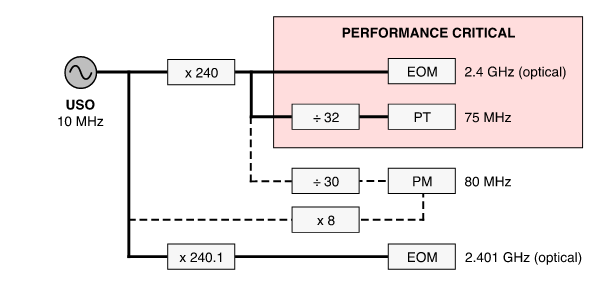
\includegraphics[width=\linewidth]{images/FDM.png}
    \caption{Clock-generation and distribution scheme highlighting performance-critical paths. A 10 MHz USO signal is multiplied to 2.4 GHz for optical sideband modulation via the \ac{EOM}, forming the primary clock-transfer tone. Parallel synthesis chains generate the 75 MHz \ac{PT} used for ADC timing correction and the 80 MHz sampling clock driving the \ac{PM}. The shaded region marks the performance-critical elements, where clock phase noise must be preserved with high fidelity. A slightly offset 2.401 GHz modulation is generated for the opposite spacecraft to produce MHz-offset sideband–sideband beat notes. The architecture ensures coherent distribution of clock noise into both optical modulation and digital sampling paths, enabling subsequent clock-noise suppression in post-processing. }
    \label{fig:fdm}
\end{figure}

%For the clock jitter terms, we can generally assume that the delay operators commute.
\begin{figure}
    \centering
    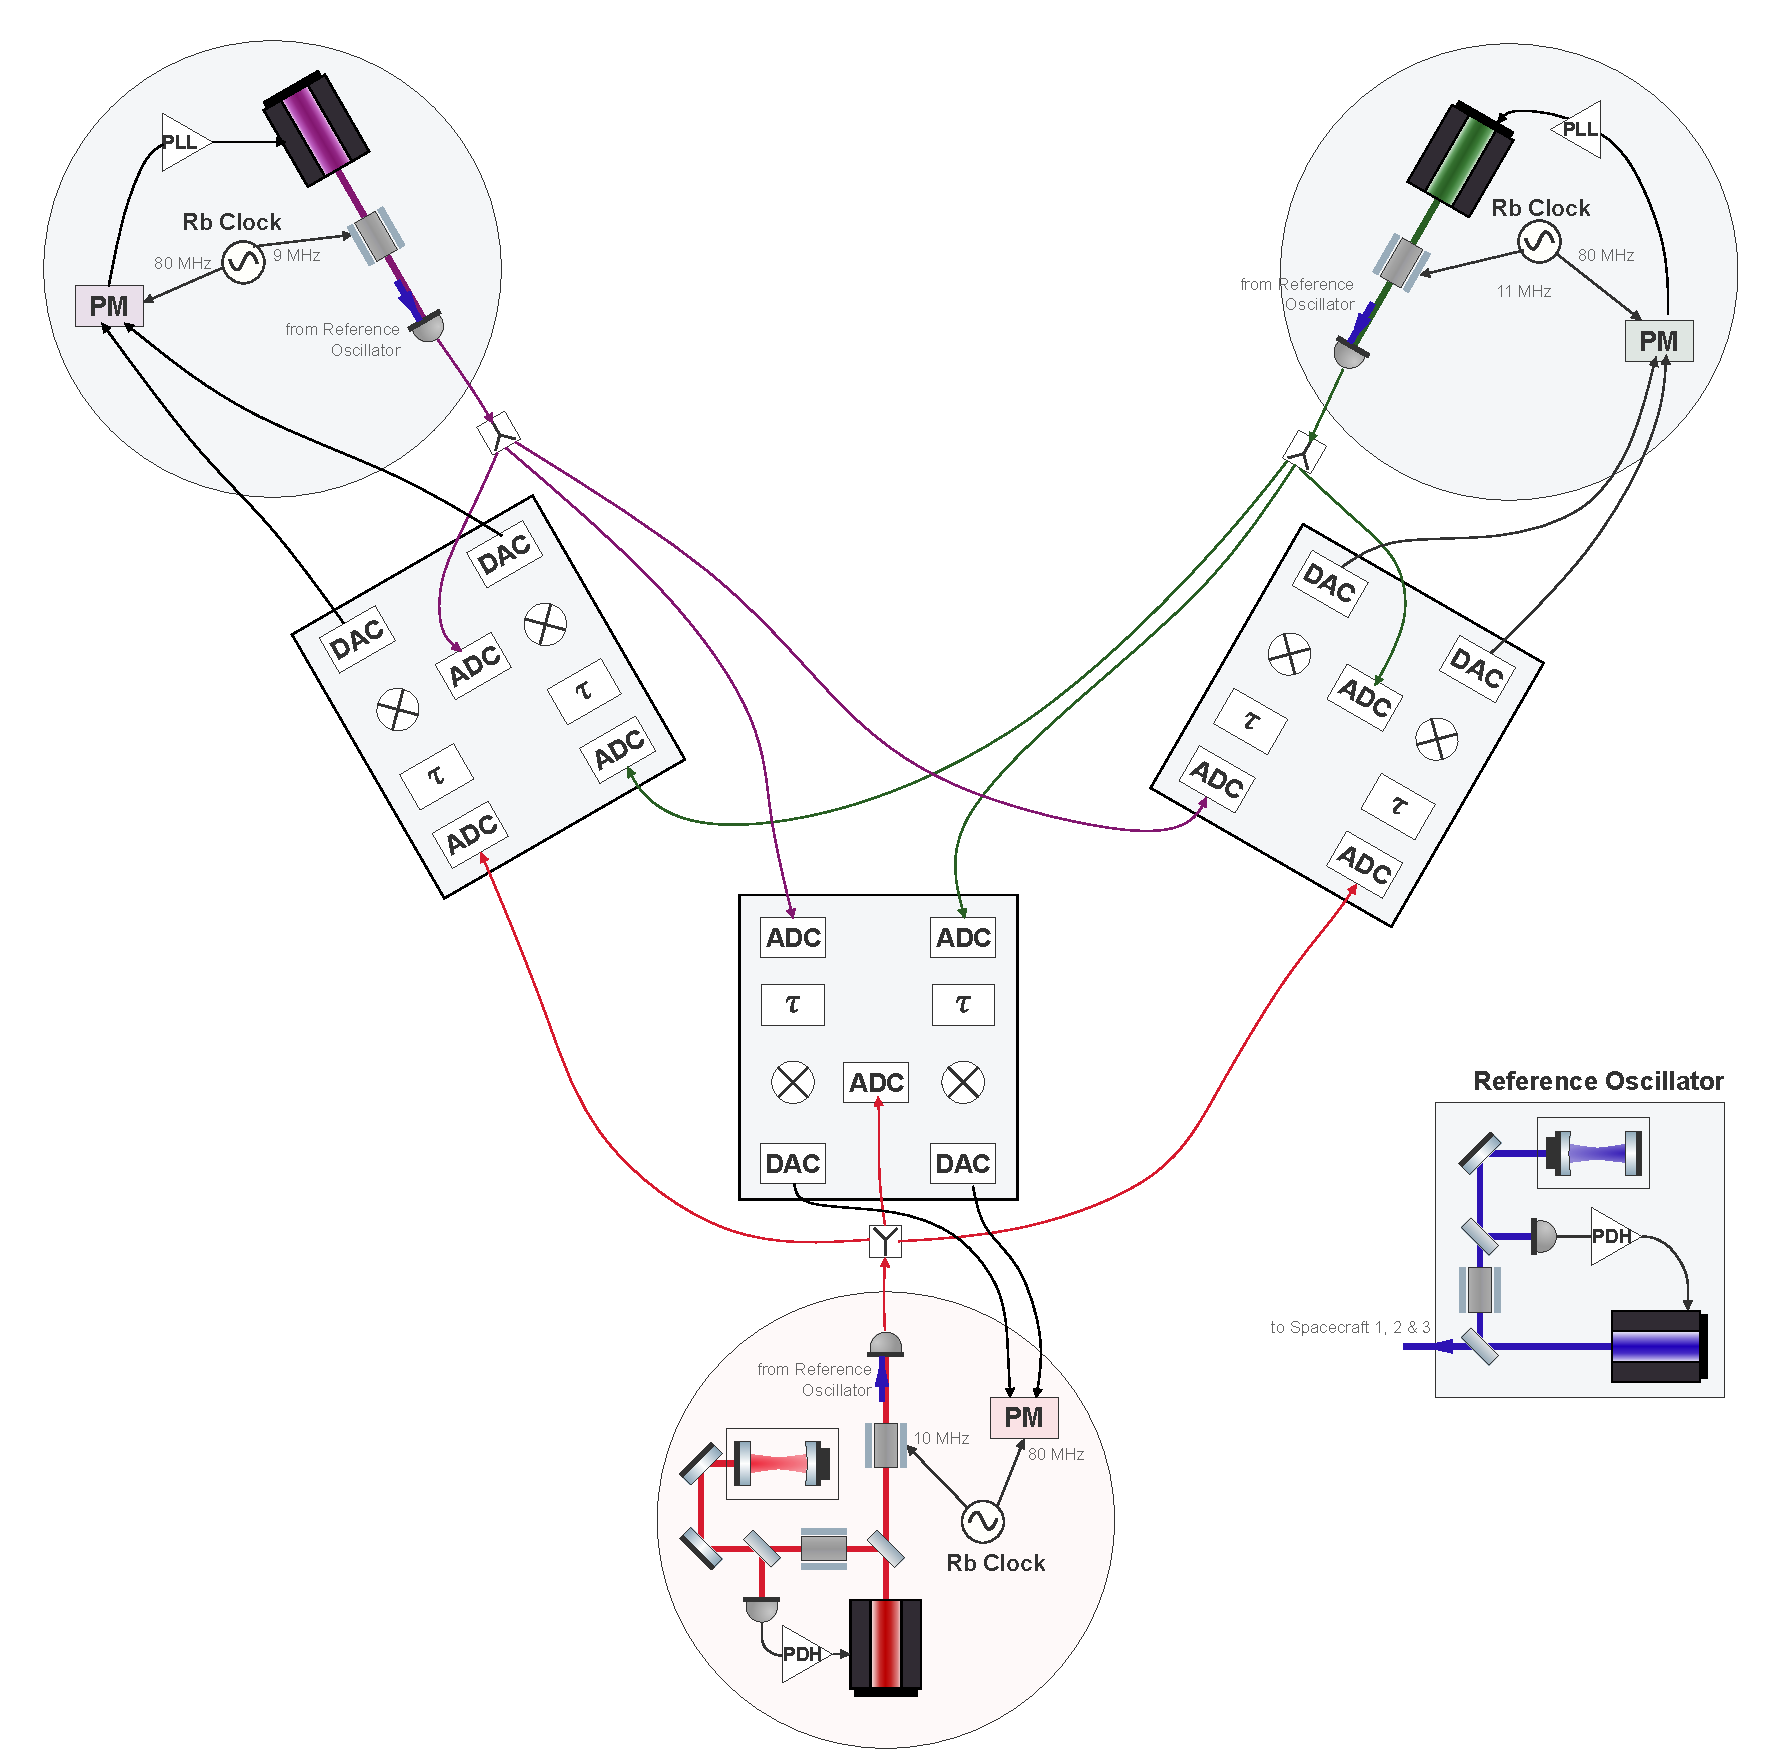
\includegraphics[width=\linewidth]{images/3arm.pdf}
    \caption{Triangular LISA testbed laboratory implementation. Three simulated spacecraft are arranged in a closed topology, each equipped with a laser, phasemeter (PM), and an independent Rb clock. The MHz heterodyne beat notes are digitised and routed through programmable delay blocks that emulate the inter-spacecraft light-travel times required for \ac{TDI}. In general, two signals are delayed on each delay-line board; these are configured to represent the incoming links to a given spacecraft, while the clock driving that delay board is matched to the corresponding spacecraft phasemeter. A common optical reference oscillator provides pre-stabilisation via PDH locking. This architecture preserves the essential structure of LISA’s one-way measurements while replacing physical arm lengths with electronic delays.}
    \label{fig:triangular}
\end{figure}
%Due to the differences in how the modulating signal vs the pilot tone on the left and right side MOSAs are derived, the correcting terms for the right side are noisier and need further corrections using the reference interferometer sideband measurements. However, as our testbed essentially implements one MOSA per spacecraft, this correction to the correcting variables can't be tested without additional hardware.

%\todo[inline]{this following section should be removed}
%\section{Previous Results}
%\subsection{Experimental demonstrations regarding TDI and clock noise transfer}
\subsubsection{JPL Interferometry Testbed (de Vine et al., 2010)}

The first reported hardware demonstration of TDI was carried out at JPL by de Vine et al. [REF]. The setup implemented a two-spacecraft configuration with two lasers per spacecraft and independent phasemeter clocks and static arm lengths of about 1 m — reproducing several of the key experimental complexities of LISA including multiple heterodyne frequencies, independent clocks, and independent phase measurements of both optical signals and clock sidebands. White noise was injected into the inter-spacecraft phase-locked loop to bring laser frequency noise to approximately 800 Hz/$\sqrt{\text{Hz}}$. The experiment demonstrated TDI suppression of laser frequency noise by roughly nine orders of magnitude and clock phase noise by about four to five orders of magnitude at 3 mHz, recovering the intrinsic displacement noise floor of the testbed at around $10^{-5}$ cycles/$\sqrt{\text{Hz}}$. One limitation was that the arm lengths were static and short, and physical light-travel times representative of the LISA constellation were not reproduced.

\subsubsection{UFLIS (Mitryk et al., 2010 and 2012)}
The University of Florida Laser Interferometry Simulator (UFLIS) was the first setup to include electronic phase delay units capable of time-varying delays on the order of seconds, allowing spacecraft motion effects to be included for the first time in a hardware TDI testbed [REF, REF]. Each spacecraft was represented by one laser: two were PDH-locked to ULE cavities, achieving a combined beatnote stability of 30–300 Hz/$\sqrt{\text{Hz}}$ near LISA pre-stabilization levels, while the remaining lasers were phase-locked to this cavity-stabilized reference with MHz offsets. The delays were applied by the Electronic Phase Delay (EPD) unit with delay rates updated continuously during a run to simulate time-changing inter-spacecraft separations. UFLIS showed suppression of pre-stabilized laser phase noise to approximately $10^{-5}$ cycles/$\sqrt{\text{Hz}}$, recovering the testbed's intrinsic noise floor, and demonstrated that second-generation TDI outperforms first-generation combinations when delays are linearly changing. GW signal injection was also demonstrated, with sinusoidal signals recovered in the TDI spectrum. Its primary limitation relative to the present work is the absence of independent clock sources: all spacecraft clocks were synchronized, meaning clock noise and its suppression via sideband transfer could not be studied.

\subsubsection{Hexagon / AEI Clock Synchronization (Yamamoto et al., 2022)}
The Hexagon interferometer at the Albert Einstein Institute in Hannover is a picometer-stable optical testbed for the LISA phasemeter, extended to simulate inter-spacecraft clock transfer by equipping each simulated spacecraft with an independent clock and GHz sideband modulation via EOMs [REF, REF]. Without clock synchronization, the three-signal combination is dominated by differential clock jitter. After applying clock synchronization via TDIR-like processing and sideband measurements, the clock noise was suppressed by three orders of magnitude at 1 Hz and up to six orders of magnitude at 0.1 mHz, bringing the residual below the LISA single-link requirement of 10 pm/$\sqrt{\text{Hz}}$ across the observation band. The post-correction floor is set by the optical bench sensitivity, which is close to but not yet at the LISA 1 pm/$\sqrt{\text{Hz}}$ single-link mark, with ongoing noise hunting to close the remaining gap. The experiment also provided the first hardware observation of several secondary noise couplings relevant to TDI: \ac{ADC} aliasing, the flexing-filtering coupling, and Lagrange interpolation error. The Hexagon does not implement programmable inter-spacecraft delays, and is therefore complementary to testbeds focused on TDI laser noise suppression. Work on Hexagon continues as it is a part of the official LISA test plan.

\subsubsection{LISA on Table / LOT (Vidal 2023, 2025)}
The LISA On Table (LOT) experiment, developed at the AstroParticule et Cosmologie (APC) laboratory in Paris, is an electro-optical simulator in which laser frequency noise and inter-spacecraft delays are generated entirely by \ac{DDS}, with no physical optical path [REF]. Clock noise and GW signal injection are not included. With DDS-generated laser noise of approximately 100$\sqrt{2}$ Hz/$\sqrt{\text{Hz}}$, both TDI 1.0 and 2.0 suppress laser frequency noise to the intrinsic testbed floor of $10^{-5}$ cycles/$\sqrt{\text{Hz}}$, consistent with other testbeds. Beyond laser noise suppression, the LOT was used to experimentally identify and characterize the non-commutativity between the delay operator and the phasemeter CIC decimation filters, producing residual aliased laser noise with a characteristic f² slope — a finding validated against an analytical model and shown to require at least a third-order CIC filter in LISA to remain below the allocated phasemeter noise level [REF].

\subsubsection{TianQin Clock Transfer (Zeng et al., 2023)}
The TianQin group at Sun Yat-sen University demonstrated inter-spacecraft clock jitter readout based on laser sideband phase transfer under weak-light conditions ($\approx$1~nW received power), with a simulated $\approx$50~µs propagation delay using a 10~km optical fiber [REF]. Each simulated spacecraft carried an independent clock — one oven-controlled crystal oscillator and one rubidium clock — with GHz sideband modulation via EOMs following the same clock transfer scheme as LISA. Comparison between electrical and optical clock transfer paths identified the GHz frequency synthesizer as the dominant noise source below 50~mHz. After differential clock noise correction, the residual optical chain noise was below 40~fs/$\sqrt{\text{Hz}}$ above 6~mHz, and carrier phase accuracy reached $10^{-4}$~cycles/$\sqrt{\text{Hz}}$ above 6~mHz, recovering the phasemeter noise floor. The experiment does not include programmable arm-length delays, TDI post-processing, or laser frequency noise, and thus addresses only the clock transfer component of the full metrology chain.

\subsubsection{HUST Picometer Signal Recovery (Xu et al., 2023)}
Xu et al.\ demonstrated combined TDI-like laser noise cancellation and clock noise removal with physical signal recovery [REF]. The setup used a single laser split through two AOMs at 75~MHz and 85~MHz to create uncorrelated effective laser noises between two simulated spacecraft, each carrying an independent clock with GHz sideband modulation via EOMs. A PZT-actuated mirror injected a 60~pm, 1~Hz displacement signal. With input laser frequency noise at approximately $10^{3}$~cycles/$\sqrt{\text{Hz}}$ and clock noise several orders of magnitude above the noise floor, the post-processing suppressed laser frequency noise by five orders of magnitude and clock noise by two orders of magnitude, recovering the 60~pm signal cleanly at the intrinsic interferometer floor of $\sim$$10^{-11}$~m/$\sqrt{\text{Hz}}$ at 1~Hz. Notably, no arm-length delay is implemented — the equal-arm geometry cancels laser noise directly — so the experiment validates signal recovery under the TDI equal-arm principle rather than testing TDI under realistic unequal delays. It does not address time-varying inter-spacecraft separations, ranging, or LISA-band performance below 1~mHz.

\section{miniLISA Design}
\label{sec:setup}

\subsection{Motivation for the Present Work}
The present work extends the electronic delay-line testbed with optical inputs and independent spacecraft clocks. It combines physical laser noise, sideband-based clock transfer, and hardware delays of several seconds, and uses component measurements to estimate the performance of the combined setup.

The electronic delays place samples acquired several seconds apart in the same interferometric measurement. This lets us test noise cancellation with independently clocked hardware, including changes in the delay caused by the hardware clock itself.

\subsection{Measurement Philosophy}
The design provides six directed links between three spacecraft, allowing LISA TDI combinations to be formed within the measurement model described below. We use the familiar Michelson $X$ for the performance analysis; it uses four of these links. The testbed reproduces the \ac{LFN}, clock-noise, and GW couplings of the LISA measurements. The first index of a link denotes the receiving \ac{SC}; source quantities carry a single spacecraft index, $\delta\phi_i$, $q_i$, and $\nu_i^m$. The target carrier phase fluctuations are
\begin{equation*}
    \delta\phi^{\mathrm c}_{ij}(t)
    =\mathbf D_{ij}\delta\phi_j(t)-\delta\phi_i(t)
    +\delta\phi^{\mathrm{GW}}_{ij}(t)-\alpha_{ij}q_i(t),
\end{equation*}
and the upper-sideband fluctuations are
\begin{align*}
    \delta\phi^{\mathrm{sb,+}}_{ij}(t)={}&
    \mathbf D_{ij}\delta\phi_j(t)-\delta\phi_i(t)
    +\delta\phi^{\mathrm{GW}}_{ij}(t)\\
    &-(\alpha_{ij}+\nu_j^m)q_i(t)+\nu_j^m\mathbf D_{ij}q_j(t).
\end{align*}
Here $\alpha_{ij}$ is the signed nominal carrier beat frequency. The sideband sampling coefficient is $\gamma_{ij}=\alpha_{ij}+\nu_j^m-\nu_i^m$; combining it with the local modulation phase gives the clock term above. Both channels use the common GW phase approximation of Section~\ref{sec:modelling}. We call a measurement \emph{LISA-like} when it reproduces these couplings. Modulation, board, and readout noises are added below.

An FPGA delay line supplies the propagation delay and the prescribed Doppler and GW frequency shifts. Heterodyning the optical fields with a common reference laser brings their phase information into the MHz range accessible to the electronics. The reference laser noise becomes part of the effective input laser noise, whose cancellation is discussed below.

The testbed omits the test-mass and reference interferometers, together with test-mass acceleration noise, optical-bench motion, backlink noise, and tilt-to-length coupling. Consequently, the local combinations $T_{ji}$ and $\xi_{ji}$ used to remove bench motion in Section~\ref{sec:modelling} are unnecessary. Identifying the two bench lasers on each spacecraft with a single source also removes the need for the reference differences $z_{ji}$. The synthesized links reproduce the three-laser structure of the $\eta$ observables, but omit the reference-interferometer clock terms proportional to $\beta_{ji}$. The clock correction tested here is therefore the reduced case of the LISA construction with those terms absent.

\subsection{Optical Input}
Three lasers represent the spacecraft, each with an independent clock driving its modulation and phase measurement. A fourth laser provides the common optical reference.
The role of the reference laser is to convert the optical phase fluctuations of each \ac{SC} laser into electronically processable heterodyne beat notes, which can then be measured by the delay line. This heterodyning step effectively downconverts the optical signals from approximately 281 THz to tens of megahertz, preserving laser frequency noise in the millihertz range of interest.
Among the \ac{SC} lasers, one is frequency-stabilized to a 25 cm \ac{ULE} glass cavity, while the reference laser is locked to a 30 cm \ac{ULE} cavity via the Pound-Drever-Hall method.
Both cavities are housed in a vacuum chamber surrounded by three layers of aluminum thermal shielding. The target is a pre-stabilized \ac{LFN} level of around 30 Hz/$\sqrt{\text{Hz}}$ in the millihertz band. The remaining two \ac{SC} lasers are PLL-locked to the synthetic LISA-like beat notes.

Each spacecraft uses an independent rubidium frequency standard as the Moku reference. The Moku supplies both the phase readout and the modulation tone driving the fiber-coupled EOM. We use $q_i$ for the timing fluctuations common to the EOM drive and the phasemeter's sampling reference. Excess noise between these paths enters the modulation and readout terms separately.

The reference laser is unmodulated in the configuration described here, so the spacecraft carrier and sidebands each beat with the reference carrier. The modulation frequency must therefore keep all three electrical beat notes within the delay-line input bandwidth. These input tones carry the optical phase and clock information; the LISA-like carrier--carrier and sideband--sideband readouts are formed by digital subtraction downstream. Modulating the reference laser is a possible extension for higher modulation frequencies, discussed in Section~\ref{sec:clock_extensions}.
The construction of a two-way arm link is illustrated in the lower panel of Fig.~\ref{fig:armlink}, alongside a simplified schematic of the corresponding LISA link showing only the functionally relevant elements. Taking the signed photodetector beat phase as \ac{SC} laser minus reference laser, the carrier signal phase before additive detector noise is
\begin{align*}
    \Phi_{\mathrm{PD},i}^{\mathrm c}(t)
    ={}&\nu_{\mathrm{R},i}t
    +\delta\phi_i^{\mathrm{eff}}(t),
\end{align*}
where $\nu_{\mathrm{R},i}$ is the signed nominal beat note frequency between the reference laser and the \ac{SC} $i$ laser, and $\delta\phi_i^{\mathrm{eff}}=\delta\phi_i-\delta\phi_{\mathrm R}$ includes their relative laser phase noise.
The upper-sideband phase is
\begin{align*}
    \Phi_{\mathrm{PD},i}^{\mathrm{sb,+}}(t)
    ={}&\left(\nu_{\mathrm{R},i}+\nu_i^m\right)t\\
    &+\delta\phi_i^{\mathrm{eff}}(t)
    +\nu_i^m q_i(t)\\
    &+\nu_i^m \tau_i^{\mathrm{mod}}(t)+\psi_i^{\mathrm{mod}}(t).
\end{align*}
Here, $\tau_i^{\mathrm{mod}}$ is timing noise added by the modulation path relative to the common reference $q_i$, while $\psi_i^{\mathrm{mod}}$ is additional modulation phase noise. Noise added only by the sampling path is included in the readout terms below.
These are the single-index counterparts of $\tau_{ij}^{\mathrm{mod}}$ and $\psi_{ij}^{\mathrm{mod}}$ in Section~\ref{clock noise}, with the same dependence on modulation frequency. We write their combined upper-sideband phase noise as
\begin{equation*}
    m_i(t)=\nu_i^m \tau_i^{\mathrm{mod}}(t)+\psi_i^{\mathrm{mod}}(t).
\end{equation*}
The lower sideband carries the opposite modulation phase, $-\nu_i^m q_i-m_i$. If its signed electrical frequency $\nu_{\mathrm R,i}-\nu_i^m$ is negative, representing it at positive frequency also reverses the measured phase sign; the clock correction below uses the upper sideband.

The photodetector output is then split and distributed across three delay-line boards. One of these boards synthesizes the local LISA-like beat note signals, the other two do so for the other two \ac{SC}. The signal routing between the boards is illustrated in Fig.~\ref{fig:triangular}.

\begin{figure}
    \centering
    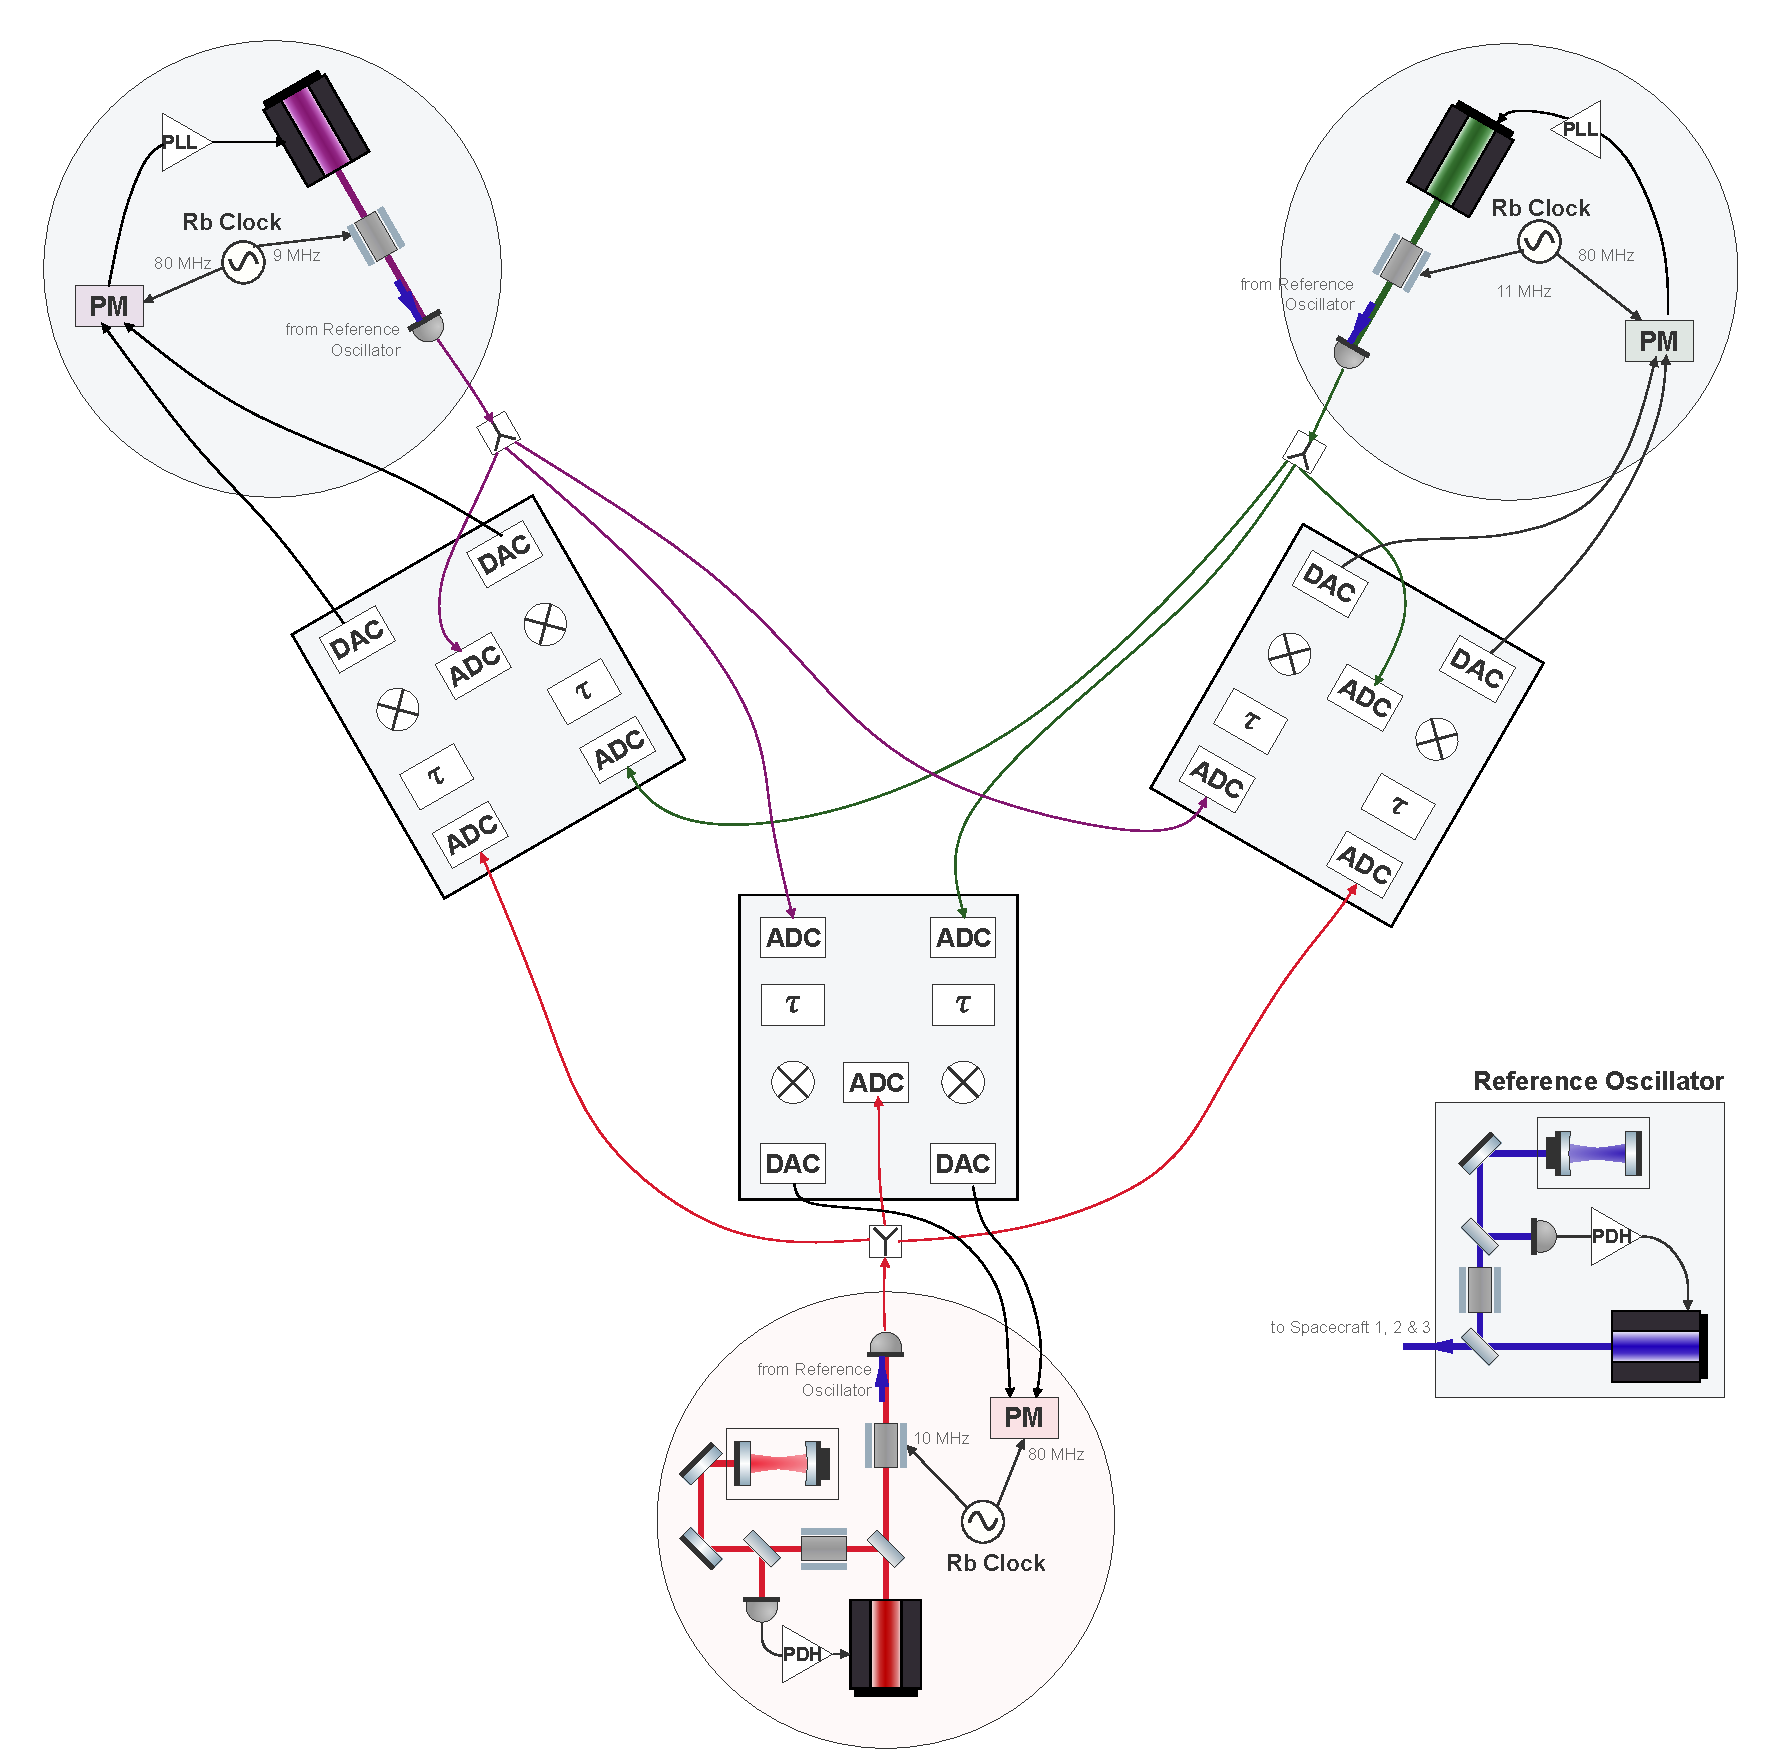
\includegraphics[width=\linewidth]{images/3arm.pdf}
    \caption{Planned six-link routing architecture for miniLISA. Each spacecraft has an optical source and an Rb-referenced Moku phasemeter that also supplies its EOM drive; each delay-line board can synthesize two incoming links. The complete routing supports six directed links, whereas the Michelson calculation in Section~\ref{sec:performance} uses links $12$, $21$, $13$ and $31$. The spacecraft-1 and reference lasers are stabilized to separate optical cavities; the other spacecraft lasers are phase-locked to synthesized beat notes. The common reference laser supplies the optical heterodyne reference.}
    \label{fig:triangular}
\reviewnote{Update the schematic labels from the legacy modulation frequencies to $(35,36,34)\,\mathrm{MHz}$ and identify the independent Rb-referenced Moku chains.}
\end{figure}


Shot noise, intensity noise and detector electronics add fluctuations to the photocurrent, which produce phase errors when the delay-line PLLs track the beat notes. Noise added before the electrical split is shared between boards; ADC and electronics noise added after the split need separate terms. Their phase-noise scales are calculated in Section~\ref{sec:readout_noise}, and their different propagation is described in Section~\ref{sec:noise_propagation}.


\subsection{The Delay Line}
\label{sec:delay_line}
The digital delay line emulates the light-travel time along each directed link. The current firmware always tracks and stores the carrier and both sidebands. At the resulting data rate, the available memory supports a maximum delay of approximately 8.5 s, covering LISA's nominal one-way light-travel time of about 8.3 s.

The implementation uses an AMD Xilinx ZCU208 RFSoC evaluation board, with integrated ADCs and DACs, FPGA programmable logic, and an embedded \ac{PS}. For each synthesized link, separate DPLLs track the carrier and sidebands of the remote and local input signals. The tracked remote frequencies are buffered to impose the arm delay, then combined with the current local frequencies. The present 125 MHz input-processing rate restricts the optical heterodyne tones to below 62.5 MHz. This is a constraint on the laboratory optical frequency plan, distinct from the frequencies of the synthesized LISA-like outputs.

Orbital delays and GW link responses are computed in advance in Python and uploaded to the \ac{PS}. During playback, the \ac{PS} converts the model inputs into fixed-point commands and streams timestamped records to the programmable logic.
The buffer supplies the macroscopic light-travel time, while fine delay actuation follows the prescribed arm-length evolution using fractional-delay interpolation. The underlying electronic architecture is described in \cite{ferguson2025applying}.

The FPGA subtracts the local frequency from the delayed remote frequency and adds the prescribed Doppler and GW offsets. Integrating this frequency produces the output phase for each of the carrier and sideband tones, which are combined at the DAC. Section~\ref{sec:gw_injection} describes the GW scaling. Omitting the nominal frequency evolution, the intended carrier phase is
\begin{equation*}
    \mathbf D_{ij}\delta\phi_j^{\mathrm{eff}}
    -\delta\phi_i^{\mathrm{eff}}+\delta\phi^{\mathrm{GW}}_{ij}.
\end{equation*}
The performance calculation below uses static delays.

The two ADC inputs and the DAC output share the timing jitter $\epsilon_i(t)$ of the board on spacecraft $i$. Sampling imprints this jitter on both inputs. The remote contribution then passes through the delay, while subtracting the local signal in the digital mixer reverses the sign of its ADC contribution. The DAC adds jitter at the output beat frequency $\alpha_{ij}$, giving
\begin{align*}
    \delta\phi^{\mathrm c}_{\epsilon,ij}(t)={}&
    -\nu_{\mathrm R,j}\mathbf D_{ij}\epsilon_i(t)\\
    &+\nu_{\mathrm R,i}\epsilon_i(t)+\alpha_{ij}\epsilon_i(t)\\
    ={}&\nu_{\mathrm R,j}(1-\mathbf D_{ij})\epsilon_i(t).
\end{align*}
Here $\alpha_{ij}=\nu_{\mathrm R,j}-\nu_{\mathrm R,i}$, so the local ADC and DAC terms combine to give $\nu_{\mathrm R,j}\epsilon_i(t)$.

The same cancellation applies to the upper sideband, with the remote input frequency replaced by $\nu_{\mathrm R,j}+\nu_j^m$:
\begin{equation*}
    \delta\phi^{\mathrm{sb,+}}_{\epsilon,ij}(t)
    =(\nu_{\mathrm R,j}+\nu_j^m)(1-\mathbf D_{ij})\epsilon_i(t).
\end{equation*}
Both expressions assume constant nominal frequencies and no additional output frequency offset.

The same board jitter also changes the physical duration of a programmed delay. For a constant command $d_{ij}$ in board time $u_i(t)=t+\epsilon_i(t)$, the input and output times satisfy $u_i(t)-u_i(t_{\mathrm{in}})=d_{ij}$. To first order,
\begin{align}
    d^{\mathrm{phys}}_{ij}(t)&=t-t_{\mathrm{in}}
      =d_{ij}+\delta d^\epsilon_{ij}(t),\\
    \delta d^\epsilon_{ij}(t)&=-(1-\mathbf D_{ij})\epsilon_i(t).
    \label{eq:board_delay_jitter}
\end{align}
Thus the physical delay can fluctuate even when its programmed value is known exactly. In LISA, ranging errors leave uncertainty in the light-travel times used for TDI. Here, board timing changes the realized delay itself. Both effects can leave laser noise if the delays applied in processing do not match the physical delays.

\subsection{GW Signal Injection}
\label{sec:gw_injection}
The GW phase defined in Eq.~\eqref{eq:gw_phase} is implemented electronically after the background delay. The required phase on the link from $j$ to $i$ is
\begin{equation*}
    \delta\phi^{\mathrm{GW}}_{ij}(t)=-\nu_jH_{ij}(t).
\end{equation*}
Since the nominal optical frequency $\nu_j$ is constant, the frequency offset supplied to the phase accumulator is
\begin{equation}\label{eq:gw_frequency_command}
    \delta\nu^{\mathrm{inj}}_{ij}(t)
    =\delta\dot\phi^{\mathrm{GW}}_{ij}(t)
    =-\nu_j\dot H_{ij}(t).
\end{equation}
Accumulating this offset reproduces the required GW phase up to an initial phase constant. The scale factor is the represented optical frequency, not the MHz beat note frequency entering the delay-line ADC. Thus the GW signal is generated by adding phase evolution to the reconstructed signal; the hardware delay itself remains $d_{ij}$ and is not additionally perturbed by $H_{ij}$. This implements the first-order propagation model of Section~\ref{sec:modelling}.

Each directed-link waveform is evaluated at its reception time $t$. The propagation and source geometry are already included in $H_{ij}$, so no additional background delay is applied to the injection waveform after it is generated. Relative timing between the playback streams must reproduce this convention.

The same GW offset is applied to the carrier and both sidebands, following the approximation in Section~\ref{sec:modelling}. It therefore cancels from their difference used for clock correction while remaining in the science signal.

When the link response is supplied as a fractional-frequency signal $y_{ij}=-\dot H_{ij}$, the command is $\delta\nu^{\mathrm{inj}}_{ij}=\nu_jy_{ij}$, using $\nu_j\simeq c/(1064\,\mathrm{nm})$ for the optical scale.
The link responses can be computed in Python for a chosen waveform and constellation geometry. Multiple sources can be combined by summing their link responses in the linear regime. The source class is not fixed by the hardware, but the resulting commands must lie within its frequency range, resolution and update bandwidth.

A signed 32-bit GW command is added on the 64-bit phase-increment scale. At a 125 MHz accumulator clock, one least significant bit corresponds to $125\,\mathrm{MHz}/2^{64}\simeq6.78\times10^{-12}\,\mathrm{Hz}$.
\reviewnote{Generate the delay commands and GW responses from the same orbit and reception-time convention. State the command update rate and verify the recovered amplitude and phase, including quantization and playback timing.}

\subsection{Readout and Data Processing}

The electrical signals produced by the delay line are digitized and tracked by Moku phasemeters, with each spacecraft's phase measurements referenced to its own clock.

The synthesized links can be used directly as $\eta$ observables. Adding in the modulation, board, and readout noises, the carrier measurement is
\begin{align*}
    \eta_{ij}(t)
    ={}&\mathbf D_{ij}\delta\phi_j^{\mathrm{eff}}(t)-\delta\phi_i^{\mathrm{eff}}(t)
    +\delta\phi^{\mathrm{GW}}_{ij}(t)
    -\alpha_{ij}q_i(t)\\
    &+\nu_{\mathrm R,j}(1-\mathbf D_{ij})\epsilon_i(t)
    +b_{ij}^{\mathrm c}(t),
\end{align*}
and the corresponding upper-sideband--upper-sideband beat note as
\begin{align*}
    \eta_{ij}^{\mathrm{sb,+}}(t)
    ={}&\mathbf D_{ij}\delta\phi_j^{\mathrm{eff}}(t)-\delta\phi_i^{\mathrm{eff}}(t)
    +\delta\phi^{\mathrm{GW}}_{ij}(t)
    -\gamma_{ij}q_i(t)\\
    &+\nu_j^m\mathbf D_{ij}q_j(t)-\nu_i^m q_i(t)\\
    &+\mathbf D_{ij}\!\left[\nu_j^m \tau_j^{\mathrm{mod}}(t)+\psi_j^{\mathrm{mod}}(t)\right]\\
    &-\nu_i^m \tau_i^{\mathrm{mod}}(t)-\psi_i^{\mathrm{mod}}(t)\\
    &+(\nu_{\mathrm R,j}+\nu_j^m)(1-\mathbf D_{ij})\epsilon_i(t)
    +b_{ij}^{\mathrm{sb,+}}(t).
\end{align*}
The terms proportional to $q_i$ describe timing common to the modulation and phasemeter reference, while those proportional to $\epsilon_i$ come from the delay-line board.

The additive phase noise $b^a_{ij}$ combines optical readout, residual board, and final-phasemeter noise, in cycles; timing and modulation noise are included explicitly. To retain the noise shared by copies of a photodetector signal, write
\begin{equation}
    b^a_{ij}=\mathbf D_{ij}p_j^a-p_i^a+e_{ij}^a,
    \label{eq:shared_readout}
\end{equation}
where $p_i^a$ is the equivalent input phase noise in channel $a$ before the split, and $e_{ij}^a$ contains noise added by the individual electronic paths. This expression assumes matched tracking responses. Any mismatch must be included in the transfer functions rather than treating copies of $p_i^a$ as independent sources.

The effective laser phases $\delta\phi_i^{\mathrm{eff}}$ enter with the same delayed-difference structure as the LISA laser phases. TDI therefore suppresses both the spacecraft and reference laser noise.

Finally, the upper-sideband-minus-carrier variable takes the form
\begin{align*}
    r_{ij}
    ={}&\frac{\eta_{ij}^{\mathrm{sb,+}}-\eta_{ij}}{\nu_j^m}\\
    ={}&\mathbf D_{ij}q_j-q_i
    +\frac{\mathbf D_{ij}m_j-m_i}{\nu_j^m}\\
    &+(1-\mathbf D_{ij})\epsilon_i
    +\frac{b_{ij}^{\mathrm{sb,+}}-b_{ij}^{\mathrm c}}{\nu_j^m}.
\end{align*}
The common GW phase cancels, leaving the clock-transfer signal together with modulation, board and readout noise.

The following common-mode cancellation assumes a shared board timing reference, with residual differences between distribution paths. Writing $\epsilon_i=\epsilon_{\mathrm{com}}+\Delta\epsilon_i$ separates their shared fluctuation from the differential jitter. In the constant-frequency model above, the common term can be absorbed into the effective laser phases and clock errors as $\delta\phi_i^{\mathrm{eff}}-\nu_{\mathrm R,i}\epsilon_{\mathrm{com}}$ and $q_i-\epsilon_{\mathrm{com}}$. It therefore cancels under TDI together with clock correction. Differential board jitter remains and sets the relevant timing residual.
\reviewnote{State which oscillator references the delay-board ADCs, DACs and delay counters, and how it is distributed. Confirm whether the boards share one reference or follow their spacecraft Rb clocks. In the latter case, specify the correlations between $\epsilon_i$ and $q_i$ and revise the timing budget accordingly.}

Table~\ref{tab:noise_comparison} summarizes the shared and laboratory-specific noise sources. The readout predictions are derived in Section~\ref{sec:readout_noise}.

\begin{table*}[t]
\centering
\caption{Noise sources shared with LISA or introduced by the miniLISA implementation, and their treatment in the present static analysis. Sources omitted from the testbed are described in Section~\ref{sec:setup}.}
\label{tab:noise_comparison}
\small
\begin{tabular}{llll}
\hline
\parbox[t]{0.19\textwidth}{\raggedright Noise source} & \parbox[t]{0.20\textwidth}{\raggedright LISA} & \parbox[t]{0.20\textwidth}{\raggedright miniLISA} & \parbox[t]{0.32\textwidth}{\raggedright Treatment / relevance} \\[5pt]
\hline
\multicolumn{4}{l}{\textbf{Present in both LISA and miniLISA}} \\[5pt]
\parbox[t]{0.19\textwidth}{\raggedright Laser frequency noise} & \parbox[t]{0.20\textwidth}{\raggedright Present} & \parbox[t]{0.20\textwidth}{\raggedright Present} & \parbox[t]{0.32\textwidth}{\raggedright Suppressed by TDI with matched delays; ideal cancellation in this estimate.} \\[5pt]
\parbox[t]{0.19\textwidth}{\raggedright Measurement-clock jitter $q_i$} & \parbox[t]{0.20\textwidth}{\raggedright Present} & \parbox[t]{0.20\textwidth}{\raggedright Present} & \parbox[t]{0.32\textwidth}{\raggedright Sideband-based post-processing correction; residual tone-generation noise remains.} \\[5pt]
\parbox[t]{0.19\textwidth}{\raggedright Modulation noise} & \parbox[t]{0.20\textwidth}{\raggedright Present} & \parbox[t]{0.20\textwidth}{\raggedright Present} & \parbox[t]{0.32\textwidth}{\raggedright Limits clock correction. Estimator assigned to source noise; channel-noise alternative remains to be tested.} \\[5pt]
\parbox[t]{0.19\textwidth}{\raggedright Science readout noise $N^{\mathrm c}_{ij}$, $N^{\mathrm{sb}}_{ij}$} & \parbox[t]{0.20\textwidth}{\raggedright Weak received light; shot noise important} & \parbox[t]{0.20\textwidth}{\raggedright Bright beams; shared detector inputs} & \parbox[t]{0.32\textwidth}{\raggedright Shared carrier noise cancels in ideal TDI; channel differences enter clock correction.} \\[5pt]
\parbox[t]{0.19\textwidth}{\raggedright ADC and phasemeter noise} & \parbox[t]{0.20\textwidth}{\raggedright Present} & \parbox[t]{0.20\textwidth}{\raggedright Present} & \parbox[t]{0.32\textwidth}{\raggedright Ideal ADC quantization included; sampling jitter and residual electronics treated separately.} \\[5pt]
\parbox[t]{0.19\textwidth}{\raggedright Delay mismatch / processing residuals} & \parbox[t]{0.20\textwidth}{\raggedright Ranging and processing errors} & \parbox[t]{0.20\textwidth}{\raggedright Board-induced delay fluctuations and processing errors} & \parbox[t]{0.32\textwidth}{\raggedright Track effective delays; only matched static delays are used in the present estimate.} \\[5pt]
\hline
\multicolumn{4}{l}{\textbf{Additional sources in miniLISA}} \\[5pt]
\parbox[t]{0.19\textwidth}{\raggedright Shared reference-laser noise} & \parbox[t]{0.20\textwidth}{\raggedright No laboratory reference laser} & \parbox[t]{0.20\textwidth}{\raggedright Present} & \parbox[t]{0.32\textwidth}{\raggedright Part of the effective source phase; suppressed by TDI in the ideal model.} \\[5pt]
\parbox[t]{0.19\textwidth}{\raggedright Delay-board timing jitter $\epsilon_i$} & \parbox[t]{0.20\textwidth}{\raggedright No electronic arm-delay board} & \parbox[t]{0.20\textwidth}{\raggedright Present} & \parbox[t]{0.32\textwidth}{\raggedright Shared jitter cancels in TDI with clock correction; differential jitter can remain.} \\[5pt]
\parbox[t]{0.19\textwidth}{\raggedright Residual delay-board electronics} & \parbox[t]{0.20\textwidth}{\raggedright No electronic arm-delay board} & \parbox[t]{0.20\textwidth}{\raggedright Present} & \parbox[t]{0.32\textwidth}{\raggedright Measured baseline included as additive noise; not assumed to cancel.} \\[5pt]
\hline
\end{tabular}
\end{table*}

\FloatBarrier
\section{Performance Modelling}
\label{sec:performance}

We estimate the noise remaining after TDI and clock correction from the measured delay-line noise, the modulation characterization and a prospective optical readout calculation. The calculation uses static delays and ideal cancellation of the common laser and clock noises.

\subsection{Noise Inputs and Comparison Reference}

For laser frequency noise we adopt the LISA pre-stabilization reference \cite{bayle_unified_2023},
\begin{equation}
 A_\nu(f)=30\,\frac{\mathrm{Hz}}{\sqrt{\mathrm{Hz}}}
 \sqrt{1+\left(\frac{2\,\mathrm{mHz}}{f}\right)^4}.
\end{equation}
Its equivalent phase ASD is $A_\phi=A_\nu/(2\pi f)$.

The clock estimate uses the phase-noise model of a 10 MHz Rb standard. Its single-sideband phase noise is anchored at $\mathcal L(10\,\mathrm{Hz})=-130\,\mathrm{dBc/Hz}$, consistent with the specifications in \cite{srs_rb_standard}. Below this point, the phase PSD is extrapolated as $f^{-1}$ down to 1 Hz, $f^{-2}$ down to 10 mHz, and $f^{-3}$ below 10 mHz. The corresponding timing ASD is
\begin{equation}
 A_q(f)=\frac{\sqrt{2\,10^{\mathcal L(f)/10}}}{2\pi\times10\,\mathrm{MHz}}.
\end{equation}
This gives approximately $2.25\,\mathrm{ps}/\sqrt{\mathrm{Hz}}$ at 10 mHz and $71\,\mathrm{ps}/\sqrt{\mathrm{Hz}}$ at 1 mHz. It is an estimate from the assumed low-frequency continuation, rather than a measurement of the laboratory clocks. The common timing noise couples to a carrier link as $|\alpha_{ij}|A_q$ and is removed by the ideal clock correction used here.

The electronic input is the measured delay-line phase-noise floor, including processing and electronics and possibly the readout phasemeter's ADC. The carrier and sideband measurements give the same floor, so we assign the same PSD to each electronic readout term. The terms are taken to be independent between links and channels, while repeated uses of a given readout remain coherent.

The modulation characterization uses half the upper-minus-lower sideband phase of a local optical beat, with a common modulation and measurement reference. The present spectrum is used as an estimate of source modulation phase noise $m_i$. The planned repeat measurement will update this input and test the proposed Moku-generated modulation tone.

Figure~\ref{fig:component_inputs_single_link} shows these component inputs in cycles/$\sqrt{\mathrm{Hz}}$. The measured spectra cover the plotted $0.25\,\mathrm{mHz}$--$1\,\mathrm{Hz}$ band without extrapolation.

For comparison, we use the single-link reference adopted in the component analysis. With $\lambda=1064\,\mathrm{nm}$, its equivalent phase ASDs are
\begin{align}
 A_{\mathrm{OMS}}(f)
 &=\frac{15\times10^{-12}\,\mathrm{m}}{\lambda}
   \sqrt{1+\left(\frac{2\,\mathrm{mHz}}{f}\right)^4},\\
 A_{\mathrm{acc}}(f)
 &=\frac{3\times10^{-15}\,\mathrm{m\,s^{-2}}}{(2\pi f)^2\lambda}
   \sqrt{1+\left(\frac{0.4\,\mathrm{mHz}}{f}\right)^2}\nonumber\\
 &\quad\times
   \sqrt{1+\left(\frac{f}{8\,\mathrm{mHz}}\right)^4}.
\end{align}
The reference is $A_{\mathrm{link}}=(A_{\mathrm{OMS}}^2+A_{\mathrm{acc}}^2)^{1/2}$. Acceleration noise is included here as a comparison quantity; it is not an experimentally present test-mass noise in the current testbed. The component spectra are displayed directly, without applying a TDI transfer function. Consequently, this figure compares input noise scales and does not establish a gravitational-wave sensitivity.

% Two-column-width variant. Use figure, width=\columnwidth, and the
% *_column.pdf filename for a single-column version.
\begin{figure*}[t]
    \centering
    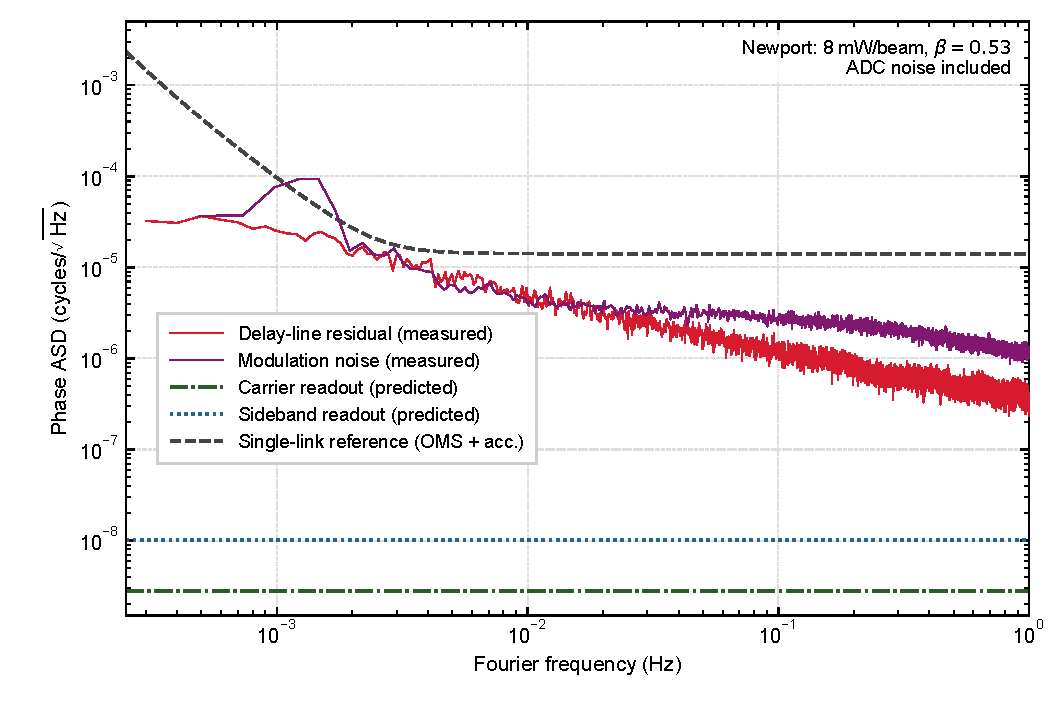
\includegraphics[width=\textwidth]{images/performance/component_inputs_single_link.pdf}
    \caption{Component phase-noise amplitude spectral densities compared with
    the single-link reference formed from optical metrology and acceleration
    noise. Solid curves show the measured delay-line residual and modulation
    phase-noise estimator; measured Fourier bins are plotted without smoothing.
    The illustrative linear-receiver carrier and first-order sideband readout noises
    include shot noise, dark-current shot noise, Johnson noise, relative
    intensity noise and ADC quantization noise. The optical model assumes one
    phase-modulated beam and one unmodulated reference beam, each delivering
    $4\,\mathrm{mW}$ at the detector, with modulation depth $0.53\,\mathrm{rad}$.
    The detector responsivity is $0.6\,\mathrm{A/W}$, heterodyne efficiency is
    $0.9$, and the termination is $50\,\Omega$ at $300\,\mathrm{K}$.
    The ADC model uses a $1\,\mathrm{V}$ full-scale span, 14 bits and
    $2\,\mathrm{GS/s}$, with an ideal three-way electrical split. The assumed white RIN is
    $0.9\times10^{-8}/\sqrt{\mathrm{Hz}}$, summed coherently between the beams.
    The model uses $(35,36,34)\,\mathrm{MHz}$ modulation and electrical carrier
    frequencies of $15.0$, $10.9$ and $21.6\,\mathrm{MHz}$; the readout
    prediction assumes white noise across the corresponding RF bands.
    All curves are shown before propagation through TDI and clock correction;
    the measured electronic residual is shown as characterized and is not
    deconvolved into individual board noise sources. The assumptions of the component budget are stated in Section~\ref{sec:performance}. }
    \label{fig:component_inputs_single_link}
\end{figure*}


\subsection{Predicted Carrier and Sideband Readout Noise}
\label{sec:readout_noise}

For the readout calculation, we consider one phase-modulated laser interfering with an unmodulated reference laser in a prospective Newport PIN-detector readout. Each beam delivers $4\,\mathrm{mW}$ at the detector, after any combining losses, and the phase-modulation depth is $\mu_{\mathrm{EOM}}=0.53\,\mathrm{rad}$. This operating mode provides an explicit carrier--carrier and sideband--carrier readout estimate. The optional configuration with both lasers modulated requires the corresponding sideband--sideband beat amplitudes to be substituted; the present numerical values should not be transferred to that mode without this adjustment.

For optical powers $P_{\mathrm{SC}}$ and $P_{\mathrm{ref}}$, responsivity $\mathcal R$, and power-overlap efficiency $\eta_{\mathrm{het}}$, the peak current of beat order $n$ is
\begin{equation}
 I_{n,\mathrm{pk}}=2\mathcal R
 \sqrt{\eta_{\mathrm{het}}P_{\mathrm{SC}}P_{\mathrm{ref}}}
 \left|J_n(\mu_{\mathrm{EOM}})\right|.
 \label{eq:perf_beat_current}
\end{equation}
The carrier uses $n=0$, and either first-order sideband uses $|n|=1$. Here $J_0(0.53)=0.9310$ and $J_1(0.53)=0.2558$. The modulated beam therefore contains $3.47\,\mathrm{mW}$ in its carrier and $0.262\,\mathrm{mW}$ in each first-order sideband. Using $\mathcal R=0.6\,\mathrm{A/W}$ and $\eta_{\mathrm{het}}=0.9$ gives peak beat currents of $4.24\,\mathrm{mA}$ and $1.16\,\mathrm{mA}$, respectively.

We include shot noise, dark-current shot noise, Johnson noise, relative intensity noise (RIN), and ADC quantization noise. Their one-sided current ASDs are modelled as
\begin{align}
 i_{\mathrm{shot}}&=\sqrt{2e[\mathcal R(P_{\mathrm{SC}}+P_{\mathrm{ref}})+I_d]},\\
 i_{\mathrm J}&=\sqrt{4k_{\mathrm B}T/R_{\mathrm L}},\\
 i_{\mathrm{RIN}}&=\mathcal R(P_{\mathrm{SC}}+P_{\mathrm{ref}})A_{\mathrm{RIN}},\\
 i_{\mathrm{ADC}}&=\frac{V_{\mathrm{FS}}}{2^{B_{\mathrm{ADC}}}G\sqrt{6f_s}}.
\end{align}
The assumed linear-receiver parameters are $I_d=100\,\mathrm{nA}$, $T=300\,\mathrm{K}$, $R_{\mathrm L}=50\,\Omega$, $G=50/\sqrt{3}\,\mathrm{V/A}$, $V_{\mathrm{FS}}=1\,\mathrm V$, $B_{\mathrm{ADC}}=14$ and $f_s=2\,\mathrm{GHz}$. The RIN ASD is $A_{\mathrm{RIN}}=0.9\times10^{-8}/\sqrt{\mathrm{Hz}}$. The RIN expression retains a conservative coherent sum of the two beams' intensity fluctuations. It represents additive noise around the RF beat frequencies; low-frequency amplitude modulation is not assumed to couple directly to phase. The ADC term uses the physical conversion rate $f_s=2\,\mathrm{GS/s}$, before the 125 MHz FPGA processing described in Section~\ref{sec:delay_line}. It assumes white quantization noise and appropriate antialias filtering; a decimated output rate is not a substitute for $f_s$ in this estimate.

The gain assumes a $50\,\mathrm{V/A}$ detector output followed by an ideal matched three-way electrical split. The split attenuates the signal and detector noise equally, while increasing the input-referred ADC contribution. At $4\,\mathrm{mW}$ per beam, the mean and maximum instantaneous optical powers are $8$ and $15.6\,\mathrm{mW}$, respectively, below the detector's listed $20\,\mathrm{mW}$ maximum \cite{newport1064}. After DC removal, the ideal phase-modulated beat has a peak-to-peak voltage of approximately $0.263\,\mathrm V$ at each ADC. These assumptions provide headroom for the prospective readout; additional RF losses are not included.

For additive noise that is locally white around the selected beat, demodulation combines noise from both RF sidebands. The equivalent phase ASD of contribution $k$ is
\begin{equation}
 A_{\phi,n}^{(k)}=\frac{\sqrt{2}\,i_k}{2\pi I_{n,\mathrm{pk}}}.
 \label{eq:perf_phase_asd}
\end{equation}
The factor $2\pi$ converts radians to cycles. No integration over the PLL bandwidth is applied to these spectral densities. Summing the component PSDs gives carrier and first-sideband readout ASDs of $3.40\times10^{-9}$ and $1.24\times10^{-8}$ cycles/$\sqrt{\mathrm{Hz}}$, respectively, equivalent to $21.4$ and $77.8\,\mathrm{nrad}/\sqrt{\mathrm{Hz}}$. Their ratio is $J_0(\mu_{\mathrm{EOM}})/|J_1(\mu_{\mathrm{EOM}})|\simeq3.64$. These are predictions for the stated optical powers and white-noise assumptions, not measurements of the complete readout chain.

\begin{figure*}[t]
 \centering
 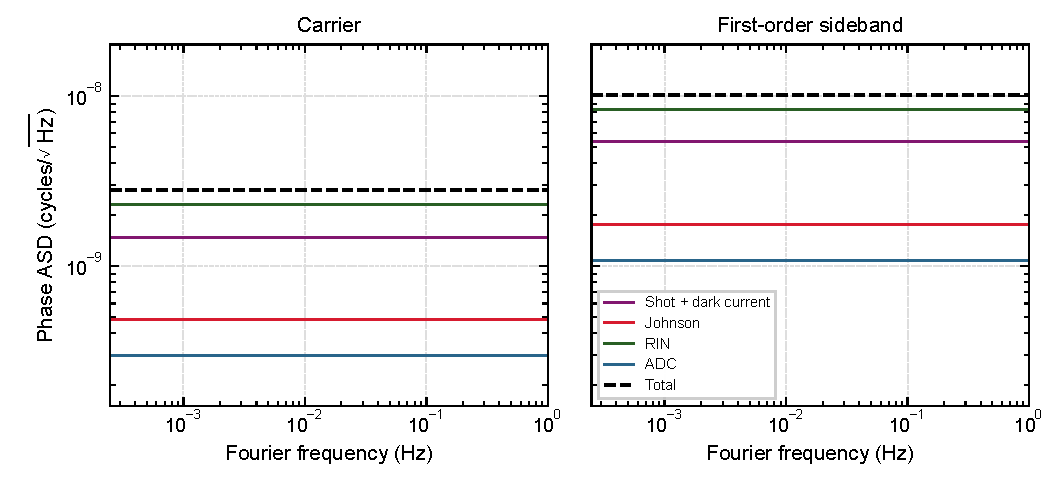
\includegraphics[width=\textwidth]{images/performance/newport_readout_breakdown.pdf}
 \caption{Illustrative linear-receiver carrier and first-order sideband readout noise for one modulated and one unmodulated beam, each delivering $4\,\mathrm{mW}$ at the detector, with modulation depth $0.53\,\mathrm{rad}$. The two panels share a common vertical scale. Shot noise includes dark-current shot noise; the ADC contribution is the white quantization estimate. The dashed curves are the quadrature totals. The beat amplitudes in Eq.~\eqref{eq:perf_beat_current} set the different phase-noise levels. The ADC estimate includes an ideal three-way electrical split.}
 \label{fig:newport_readout}
\end{figure*}

The signal levels explain why this readout operates differently from LISA's. The $4\,\mathrm{mW}$ laboratory beams produce strong carrier and sideband beats, whereas LISA must measure light received after propagation over millions of kilometres. miniLISA therefore has a much lower predicted detector readout noise than the LISA science-interferometer allocations, as summarized in Table~\ref{tab:noise_comparison}.

The testbed does not need to reproduce LISA's weak-light, shot-noise-limited readout to test laser- and clock-noise suppression. A lower readout floor makes smaller residuals from the delay and clock-transfer chains accessible. Shot noise is included in the calculation. The measured electronic residual and sideband-difference estimator exceed the calculated input readout noise; their contributions to the corrected observable depend on the source propagation discussed below. Thus the laboratory signal powers are chosen to support the noise-suppression tests, rather than to reproduce the mission's photon budget.

The LISA allocations (IRD2--IDS--04010 and IRD2--IDS--04580) increase towards low frequencies as $\sqrt{1+(f_k/f)^4}$, with $f_k=2\,\mathrm{mHz}$ for the carrier and $0.7\,\mathrm{mHz}$ for the sidebands. They refer to individual readouts and are distinct from the total OMS-plus-acceleration comparison curve used above.

These input noise levels do not by themselves specify the output noise after TDI. In particular, detector noise shared by the split input paths and noise added independently by each board have different transfer functions.

\subsection{Propagation Through TDI and Clock Correction}
\label{sec:noise_propagation}

The propagation calculation uses the four links of Michelson $X$, static delays and constant nominal frequencies. The illustrative frequency plan is $\nu_{\mathrm R,i}=(15.0,10.9,21.6)\,\mathrm{MHz}$ and $\nu_i^m=(35,36,34)\,\mathrm{MHz}$, giving $(\alpha_{12},\alpha_{21},\alpha_{13},\alpha_{31})=(-4.1,4.1,6.6,-6.6)\,\mathrm{MHz}$. The nominal one-way delay is $L=2.5\times10^9\,\mathrm m/c\simeq8.339\,\mathrm s$. These are example operating frequencies. The small modulation-frequency offsets separate the synthesized carrier and sideband beats; the laboratory readout is not constrained to the representative LISA 5--25 MHz band.
Writing $z_{ij}=\exp(-2\pi\mathrm i f d_{ij})$, $A=z_{12}z_{21}$ and $B=z_{13}z_{31}$, the static Michelson defined above becomes
\begin{align}
 X={}&(1-A)(\eta_{13}+z_{13}\eta_{31})\nonumber\\
     &-(1-B)(\eta_{12}+z_{12}\eta_{21}).
\end{align}
Let $P_{ij}$ denote its four link coefficients and $K_{ij}$ the clock-correction coefficients, chosen so that
\begin{equation}
 X_{\mathrm c}=\sum_{ij}(P_{ij}\eta_{ij}+K_{ij}r_{ij})
\end{equation}
has zero coefficient for each $q_i$. The sum runs over links $12$, $21$, $13$ and $31$, using the upper-sideband-minus-carrier definition of $r_{ij}$ given above. The static second-generation convention used in the calculation is $X_{2\mathrm c}=(1-AB)X_{\mathrm c}$; this extra filter must multiply both the science and correction weights. Laser and clock cancellation can be checked algebraically for unequal static delays. The calculation is restricted to static arms.

For four independent link noises with the same ASD $A_e$, the uncorrected TDI output is
\begin{equation}
 A_{X,e}=A_e\sqrt{\sum_{ij}|P_{ij}|^2}.
\end{equation}
Four unit-weight terms would give $\sqrt{4}A_e=2A_e$. TDI also contains delayed differences, so its weights depend on Fourier frequency. For equal delays $d$, the static $X_2=(1-AB)X$ convention gives $A_{X_2,e}=8|\sin(2\pi fd)\sin(4\pi fd)|A_e$ before clock correction.

For noise added to individual links, repeated appearances of one readout must be combined coherently. In particular, for the first-generation weights the coefficients are
\begin{equation}
 T_{b^{\mathrm c}_{ij}}=P_{ij}-\frac{K_{ij}}{\nu_j^m},\qquad
 T_{b^{\mathrm{sb,+}}_{ij}}=\frac{K_{ij}}{\nu_j^m}.
\end{equation}
The two appearances of a given carrier noise are therefore combined before taking a squared magnitude. These coefficients apply directly to $e^a_{ij}$ in Eq.~\eqref{eq:shared_readout}, not to independent copies of a shared detector noise.

For matched paths, the shared carrier term $\mathbf D_{ij}p_j^{\mathrm c}-p_i^{\mathrm c}$ has the laser-noise structure and cancels in carrier TDI. However, define the detector channel difference $\chi_i=p_i^{\mathrm{sb,+}}-p_i^{\mathrm c}$. It contributes to the clock-transfer variable as
\begin{equation}
 r_{ij}^{\mathrm{det}}=\frac{z_{ij}\chi_j-\chi_i}{\nu_j^m},
\end{equation}
and hence to the corrected observable as
\begin{equation}
 X_{2\mathrm c}^{\mathrm{det}}=(1-AB)\sum_{ij}K_{ij}
 \frac{z_{ij}\chi_j-\chi_i}{\nu_j^m}.
 \label{eq:detector_clock_residual}
\end{equation}
For the estimate, detector noise in the carrier and sideband channels is taken to be independent, so $S_{\chi_i}=S_{p_i^{\mathrm{sb,+}}}+S_{p_i^{\mathrm c}}$. Copies of each detector channel shared between boards retain the same noise realization.

 For independent physical sources $n_a$, the output PSD is
\begin{equation}
 S_{X_{2\mathrm c}}(f)=\sum_a|T_a(f)|^2 S_a(f).
\end{equation}
The measured electronic spectrum is propagated with the carrier and sideband coefficients above. The predicted detector terms use Eq.~\eqref{eq:detector_clock_residual}. ADC quantization is shown in the input readout estimate but is not added separately to the total, where electronics are represented by the measured delay-line floor.

True source modulation noise survives clock correction. At fixed nominal beat frequencies, increasing all $\nu_i^m$ by a common factor $s$ reduces its transfer coefficients by $1/s$. The output modulation ASD therefore decreases by $1/s$ for fixed direct phase noise. For fixed timing noise, the input modulation phase ASD increases by $s$, leaving the residual unchanged. These scaling statements apply to the identified physical source, not automatically to the full measured sideband-difference spectrum. Likewise, a small raw TDI ASD at low Fourier frequency partly reflects the differencing response of the observable, which also acts on a gravitational-wave signal; it is not by itself an improvement in sensitivity.

\subsection{Estimated Residual Noise}

Figure~\ref{fig:total_tdi2_noise} combines the electronic, modulation and detector contributions after static second-generation TDI and clock correction. Each physical source is multiplied by its transfer function before the output PSDs are summed. The calculation uses four independent electronic link readouts per channel and three shared detector inputs, with the assumptions given above. The detector contribution is small compared with the measured electronic and modulation inputs, consistent with the use of bright laboratory beams rather than a weak-light readout.

\begin{figure*}[t]
 \centering
 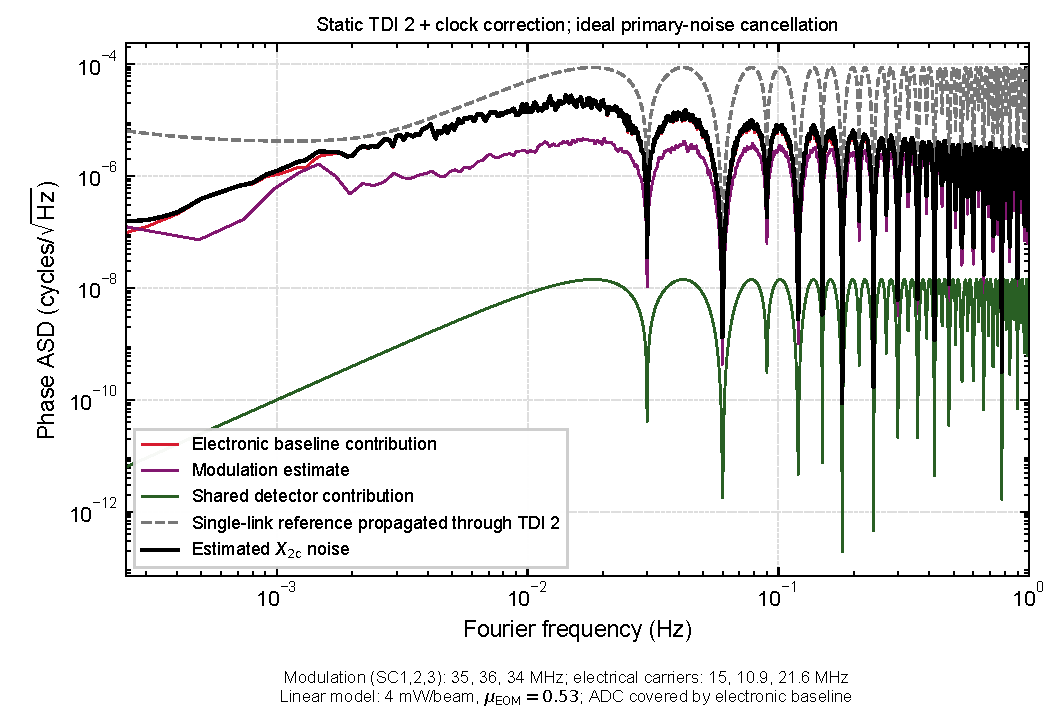
\includegraphics[width=\textwidth]{images/performance/total_noise_tdi2_corrected_budget.pdf}
 \caption{Estimated phase-noise ASD of the clock-corrected static Michelson observable $X_{2\mathrm c}$. The black curve sums the electronic, modulation and shared-detector contributions in quadrature. The calculation uses four links with $8.339\,\mathrm s$ delays, modulation frequencies $(35,36,34)\,\mathrm{MHz}$, and the optical operating point of Section~\ref{sec:readout_noise}. ADC noise is represented by the measured electronic baseline. The dashed comparison curve treats the single-link OMS-plus-acceleration reference as independent equivalent link noises propagated through the same TDI observable. Laser and common clock noise cancel ideally in this static estimate.}
 \label{fig:total_tdi2_noise}
\end{figure*}

The estimate uses the current modulation spectrum, which will be replaced after the planned repeat measurement. It describes the included component noises under ideal primary-noise cancellation, rather than a measured sensitivity of the assembled optical testbed.

Board timing also changes the physical delay, even when the programmed delay is known exactly. For constant $d_{ij}$, Eq.~\eqref{eq:board_delay_jitter} gives
\begin{equation}
 A_{\delta d^\epsilon_{ij}}(f)
 =2|\sin(\pi f d_{ij})|A_{\epsilon_i}(f).
\end{equation}
The common board timing cancels in the linear model discussed above; differential timing can remain. Its nominal beat-frequency coupling is already included in the $\epsilon_i$ terms and is not a separate independent ranging noise. No additional timing or delay-error floor is assigned in the present estimate.

Under the common carrier/sideband GW approximation, the injected signal in this static observable is
\begin{equation}
 X_{2\mathrm c}^{\mathrm{GW}}=(1-AB)\sum_{ij}P_{ij}\delta\phi^{\mathrm{GW}}_{ij}.
\end{equation}
This provides the amplitude and phase prediction for a subsequent hardware injection test.



\section{Future Extensions}
%\subsection{Discussion on Omitted noise sources }
%We omit noise sources associated with the test mass, including test-mass acceleration noise and optical-bench jitter, as the testbed does not include the gravitational reference sensor. Backlink noise, arising from the fiber connecting the two optical benches on a given spacecraft, is similarly absent from the current configuration.
\subsection{Injection of Secondary Noise}
Test-mass displacement can be emulated by adding the corresponding phase terms $M_{ij}$ from Section~\ref{sec:modelling} to the synthesized links. Each simulated test mass must use the same displacement realization wherever it occurs, including the delayed occurrence in the reverse link. Independent noise added to every link would not reproduce these correlations. For a specified acceleration spectrum, the displacement ASD is obtained by dividing by $(2\pi f)^2$ over the analysis band. This injection would test the secondary-noise transfer functions as well as primary-noise suppression.

Independent phase perturbations can also be added after link synthesis to test a prescribed LISA-like readout-noise model. Lower optical power would test weak-light tracking and readout, but would not by itself remove the correlations introduced by splitting one detector output across boards.

\subsection{Time-Dependent Delays}
The six-link design supports TDI combinations beyond the four-link Michelson considered here. Orbit-derived delays and Doppler shifts would extend the present static analysis to arm flexing and second-generation TDI. The analysis here uses phase data. For a time-dependent delay, differentiation gives
\begin{equation}
 \frac{d}{dt}\bigl[\mathbf D_{ij}\delta\phi_j\bigr]
 =(1-\dot d_{ij})\mathbf D_{ij}\delta\dot\phi_j.
\end{equation}
Thus frequency-domain measurements require Doppler-weighted delay operators \cite{bayle_adapting_2021}. In this hardware, buffering tracked frequency and adding a nominal Doppler offset does not by itself supply the factor multiplying the fluctuating frequency.
\reviewnote{Check whether the firmware scales the delayed frequency fluctuations by $1-\dot d_{ij}$. Implement this factor or quantify the deviation before claiming an orbit-consistent phase response. Use the represented optical frequency for the nominal Doppler shift, and rederive the board-jitter coefficients with the actual output frequency.}
\reviewnote{For a full TDI-2 analysis, use ordered, nested delays and time-dependent carrier and sideband clock coefficients, then verify the corresponding clock correction. Give a TDI-1 flexing residual for the selected orbit and compare it with TDI-2; the static filter $(1-AB)$ alone does not demonstrate flexing-arm cancellation.}
\reviewnote{Specify delay-command update rates, accumulator precision, interpolation error and logging of realized delays. Check the maximum commanded delay against the 8.5 s memory limit. Describe time-frame alignment and whether processing delays are commanded, logged or fitted by TDI ranging, including clock and cable offsets.}
\reviewnote{Develop and validate a frequency plan over the chosen orbit: all three output tones must remain trackable without zero crossings or overlap. A digital output offset changes sampling-clock and DAC-jitter couplings and must be included explicitly in both carrier and sideband coefficients; it is not automatically equivalent to an optical frequency-plan change.}

\subsection{Changes to the Clock-Transfer and Locking Configuration}
\label{sec:clock_extensions}
Changing the modulation frequency requires separating the measured estimator into modulation, timing and readout contributions, as discussed in Section~\ref{clock noise}. A GHz implementation would also require a compatible optical and RF frequency plan. Modulating the reference laser would allow corresponding optical sidebands to beat within the electronic input band.

A second optical source and modulator on each spacecraft, together with reference interferometers and backlinks, would reproduce the local $\xi/z/\eta$ reduction and the $\beta$ clock couplings omitted here \cite{otto2012tdi}. Distinct synthesis chains and a local sideband comparison would also allow tests of differential tone-generation noise.



\begin{comment}
\begin{table*}[htbp]
\centering
\caption{Comparison of key metrology elements between LISA and the present testbed.}
\label{tab:lisa_testbed_comparison}
\begin{tabular}{lcc}
\hline
\textbf{Element} & \textbf{LISA} & \textbf{Testbed} \\
\hline
Lasers per spacecraft
& 2
& 1 \\

Laser pre-stabilisation
& Optical cavity, phase locking
& Optical cavity, phase locking \\

Inter-spacecraft links
& Optical (free-space)
& Electrical (after heterodyning) \\

Delay implementation
& Physical light-travel time
& FPGA-based electrical delay line \\

Delays
& 8.3 s
& 8.3 s\\

Ranging
& PRN
& tone assisted \\

Clock sources
& 3 independent USOs
& 3 independent USOs \\

Clock transfer
& GHz sideband modulation
& MHz sideband modulation \\

Reference interferometer
& Implemented
& not presently implemented \\


TDI generation considered
& Second generation
& First generation, Second in the future \\

\hline
\end{tabular}
\end{table*}

\end{comment}




\section{Conclusion}\label{Conclusion}
We have presented the miniLISA design, which extends an electronic delay-line testbed with optical sources and independently referenced spacecraft measurements. Building on hardware demonstrations with electronic propagation delays \cite{mitryk_hardware-based_2012,ferguson2025applying}, it is intended to test laser-noise suppression, a reduced clock-transfer model, and GW signal recovery within the same measurement chain.

The estimate combines the measured electronic and modulation spectra with a prospective detector readout model, using the appropriate source and link transfer functions. Bright laboratory beams keep the predicted photodetector readout noise below the LISA science-interferometer allocations. Board timing introduces an additional coupling, including fluctuations of the effective delay, whose residual depends on differential board jitter and the delays used in processing. This component estimate provides a reference for the performance of the assembled optical testbed.

The next steps are to repeat the modulation-noise measurement, assemble the optical readout, and test noise suppression and GW recovery with the six-link setup. Varying delays and higher modulation frequencies would extend these tests.

%\newpage
%\listoftodos[Notes]

% Definitions only - not typeset, see the nolist option in the preamble.
\begin{acronym}
    %\acro{AC}{alternatng current}
    \acro{ADC}{analog to digital converter}
    \acro{EOM}{electro-optic modulator}
    \acro{DAC}{digital to analog converter}
    \acro{DDS}{direct digital synthesis}
    \acro{DPLL}{digital phase lock loop}
    \acro{FDS}{frequency distribution system}
    \acro{FPGA}{field programmable gate array}
    \acro{GW}{gravitational wave}
    \acro{IDS}{interferometric detection system}
    %\acro{ISI}{interspacecraft interferometer}
    \acro{LISA}{Laser Interferometer Space Antenna}
    \acro{LFN}{laser frequency noise}
    \acro{LVK}{LIGO-Virgo-KAGRA}
    \acro{MOSA}{movable optical system assembly}
    %\acro{PD}{photodetector}
    %\acro{PDH}{Pound-Drever-Hall}
    \acro{PLL}{phase locked loop}
    \acro{PM}{phasemeter}
    \acro{PMS}{phase measurement system}
    \acro{PS}{processsing unit}
    \acro{PT}{pilot tone}
    \acro{SC}{spacecraft}
    \acro{TDI}{time delay interferometry}
    \acro{UFLIS}{University of Florida Laser Interferometry Simulator}
    \acro{ULE}{ultra-low expansion}
    \acro{USO}{ultra-stable oscillator}
\end{acronym}

\newpage
% unsrt numbers references in order of first citation in the text
% (plain would sort them alphabetically by author instead).
\bibliographystyle{unsrt}
\bibliography{citations}

%\appendix


\end{document}
